%\documentclass{book}\usepackage{sjtfonts}\usepackage{includegraphics}\usepackage{alltt}\usepackage{latexsym}
%\usepackage{array}
%\begin{document}\input{defs0}%		miradefs.tex 		    June 1994

% opening and closing a quoted Miranda section

\newcommand{\mira}{\noindent\hrulefill\nopagebreak\so}
\newcommand{\arim}{\nopagebreak\st\hrulefill\\}

% backslash in the Miranda environment
% Only feasible approach is to use \verb+\+
% in line!

%\newcommand{\bs}{$\mi\backslash\!\!$}
%\newcommand{\lbs}{\mbox{\verb+\+}}

% ignoring part of the input

\newcommand{\ignore}[1]{}

% a blank line in a Miranda section

\newcommand{\bl}{\mbox{\ }}

% Signalling a diffculty.

\definecolor{light-gray}{gray}{0.95}

\newcommand{\beware}[2]
 {\medskip\noindent\colorbox{light-gray}{\parbox{\textwidth}
 {\mbox{\large\textbf{#1}} \medskip\noindent\\ #2}\medskip\noindent}}

% Subscripting in Miranda text
\newcommand{\subscr}[2]{\mbox{${\mbox{\texttt{#1}}}_{\mbox{\texttt{#2}}}$}}

%\newcommand{\subscr}[2]{\mbox{${\mbox{\mi #1}}_{\mbox{\smtt #2}}$}}
\newcommand{\aone}{\subscr{a}{1}}
\newcommand{\atwo}{\subscr{a}{2}}
\newcommand{\ak}{\subscr{a}{k}}

\newcommand{\aoneone}{\subscr{a}{1,1}}

\newcommand{\eone}{\subscr{e}{1}}
\newcommand{\etwo}{\subscr{e}{2}}
\newcommand{\ei}{\subscr{e}{i}}
\newcommand{\er}{\subscr{e}{r}}

\newcommand{\fone}{\subscr{f}{1}}
\newcommand{\fl}{\subscr{f}{l}}

\newcommand{\gone}{\subscr{g}{1}}
\newcommand{\gtwo}{\subscr{g}{2}}
\newcommand{\gi}{\subscr{g}{i}}
\newcommand{\gr}{\subscr{g}{r}}

\newcommand{\hone}{\subscr{h}{1}}
\newcommand{\hl}{\subscr{h}{l}}

\newcommand{\pone}{\subscr{p}{1}}
\newcommand{\ptwo}{\subscr{p}{2}}
\newcommand{\pk}{\subscr{p}{k}}

\newcommand{\qone}{\subscr{q}{1}}
\newcommand{\qtwo}{\subscr{q}{2}}
\newcommand{\qk}{\subscr{q}{k}}

\newcommand{\rone}{\subscr{r}{1}}
\newcommand{\rtwo}{\subscr{r}{2}}

\newcommand{\tone}{\subscr{t}{1}}
\newcommand{\ttwo}{\subscr{t}{2}}
\newcommand{\tn}{\subscr{t}{n}}

\newcommand{\vone}{\subscr{v}{1}}
\newcommand{\vtwo}{\subscr{v}{2}}
\newcommand{\vn}{\subscr{v}{n}}

% for regular expressions

\newcommand{\stone}{\subscr{st}{1}}
\newcommand{\sttwo}{\subscr{st}{2}}
\newcommand{\stn}{\subscr{st}{n}}
\newcommand{\rthree}{\subscr{r}{3}}

\newcommand{\eps}{$\varepsilon$}
\newcommand{\trans}[1]{\stackrel{\mbox{\tt #1}}{\longrightarrow}}



% superscript in Miranda text

\newcommand{\superscr}[2]{\mbox{${\mbox{\mi #1}}^{\mbox{\smtt #2}}$}}

% Not equals in Miranda text

\newcommand{\noteq}{\makebox[0pt][l]{=}/}
\newcommand{\overslash}{\makebox[0pt][l]{/}}

% Definitions in complexity chapter

\newfont{\oldSym}{cmsy10}
\newcommand{\Th}{\boldmath$\oldSym\Theta$}
\newcommand{\pow}[1]{\^{}#1}
\newcommand{\leqq}{$\leq$}
\newcommand{\geqq}{$\geq$}
\newcommand{\lll}{$\ll$}
\newcommand{\eqq}{$\equiv$}
\newcommand{\ltwo}{\subscr{log}{2}}

% Indexing

\newcommand{\minx}[1]{\index{#1@{\ttfamily{}#1}}}
\setcounter{chapter}{15}\setcounter{page}{287}

\chapter{Abstract data types}
\chapstart
\label{adt}
\index{abstract data type|(}
\index{abstract data type!sets|see{sets}}
\index{abstract data type!store|see{store}}

The Haskell module system allows definitions of functions and other objects to
be hidden when one module is imported into another. Those definitions
hidden are only of use in defining the exported functions, and hiding them
makes clearer the exact interface between the two modules: only those features
of the module which are needed will be visible.

This chapter shows that information hiding is equally applicable for types,
giving what are known as \textbf{abstract data types}, or \textbf{ADT}s. We explain the abstract data type 
mechanism here, as well as
providing a number of examples of ADTs, including queues, sets, relations and the fundamental
types belonging to a simulation case study.
\minx{module}\minx{type}

\section{Type representations}

We begin our discussion with a scenario which is intended to show both the
purpose and the operation of the abstract data type mechanism.

Suppose we are to build a calculator for numerical expressions, like those
given by the \texttt{Expr}\minx{Expr} type of Section \ref{recTypes}, but with variables
included.
The calculator is to provide the facility to set the values of variables, as
well as for variables to form parts of expressions. 

As a part of our system, we need to
be able to model the current values of the variables, which we might call the
\textbf{store} of the calculator. How can this be done? A number of models
present themselves, including:\index{store}\index{case
studies!calculator|see{calculator}}\index{calculator|(}
\begin{titemize}
\item a list of integer/variable pairs: \texttt{[(Integer,Var)]}; and
\item a function from variables to integers: \texttt{(Var -> Integer)}.
\end{titemize}
Both models allow us to look up and update the values of variables, as well
as set a starting value for the store. These operations have types as
follows. 
\begin{alltt}\minx{initial}\minx{value}\minx{update}
initial :: Store
value   :: Store -> Var -> Integer  \hfill(StoreSig)\minx{Store}
update  :: Store -> Var -> Integer -> Store
\end{alltt}
but each model
allows more than that: we can, for instance, reverse a list, or compose a
function with others. In using the type \texttt{Store} we intend
only to use the three operations given, but it is always possible to use the
model in unintended ways.

How can we give a better model of a store? The answer is to define a
type which \textbf{only} has the operations \texttt{initial}, \texttt{value} and
\texttt{update}, so that we cannot abuse the representation. We
therefore hide the information about how the type is actually
implemented, and only allow the operations \texttt{(StoreSig)} to manipulate objects
of the type. 

When we provide a limited interface to a type by means of a specified set
of operations we call the type an \textbf{abstract data type} (or ADT).
\index{ADT|see{abstract data type}} 
Since the
`concrete' type itself is no longer accessible and we
may only access the type by
means of the operations provided, these operations give a more `abstract'
view of the type.

\begin{figure}[t]
\begin{center}
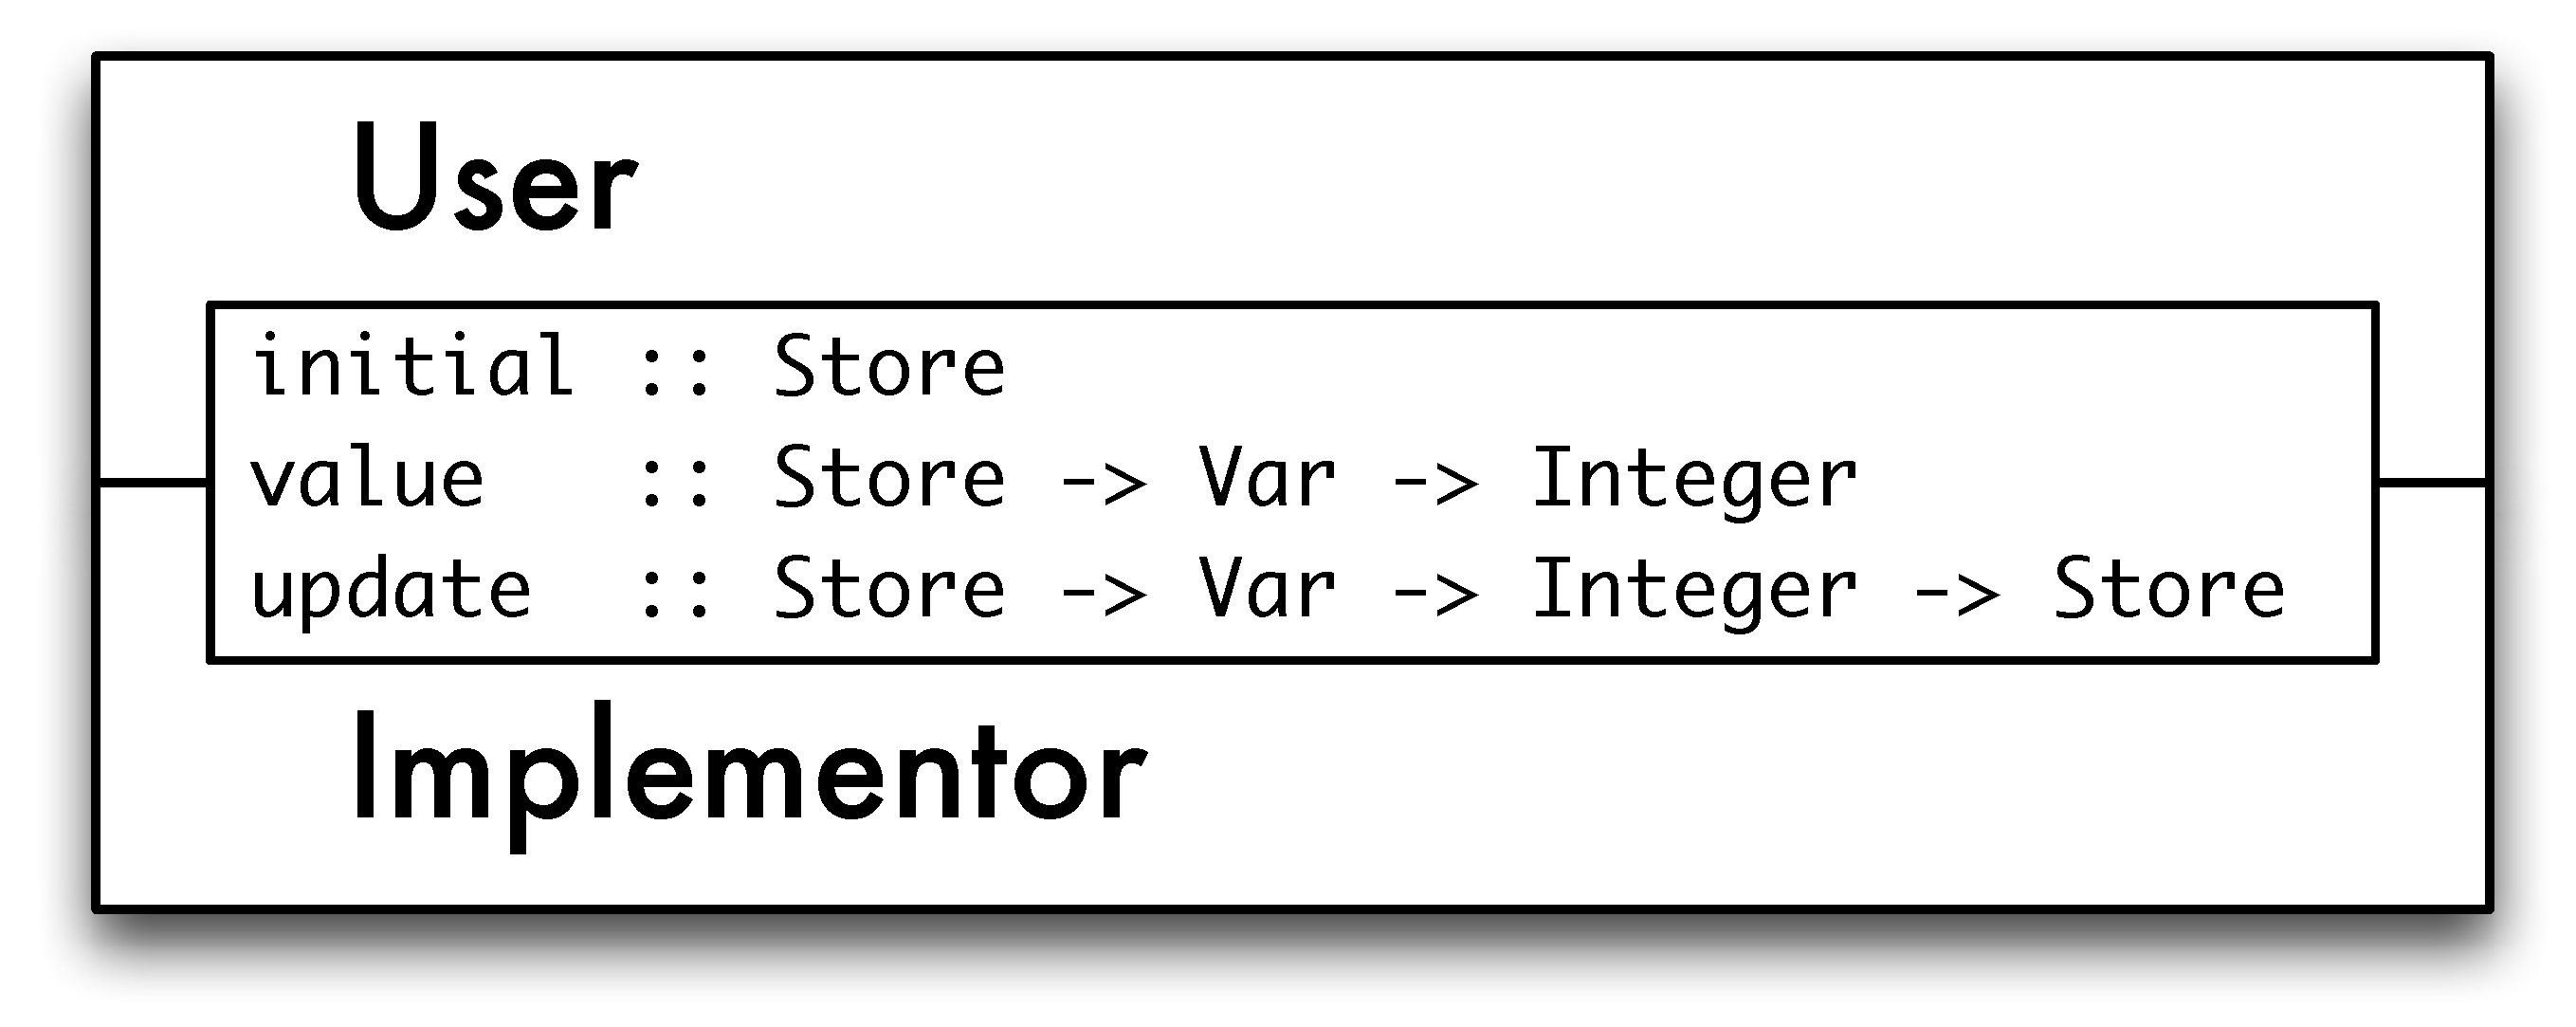
\includegraphics[width=3.5in]{Pictures/StoreADT.pdf}
\end{center}
\caption{The \texttt{Store} abstract data type.}
\label{storePic}
\end{figure}
Figure \ref{storePic} illustrates the situation, and suggests that as
well as giving a natural representation of the type of stores, there are
two other benefits of type abstraction.
\begin{titemize}
\item The type declarations in \texttt{(StoreSig)} form a clearly defined {\bf
interface},
\index{interface}
which is called the {\bf
signature}\index{signature}\index{abstract data type!signature} of the ADT, 
between the user of the type and its implementer. The only information that
they have to agree on is the signature; once this is agreed, they can work
independently. This is therefore another way of breaking a complex problem
into simpler parts; another aspect of the
`divide and conquer' method. \index{divide and conquer}
\item We can \textbf{modify} \index{program modification}the implementation of the \texttt{Store} without
having any effect on the user. Contrast this with the situation
where the implementation is visible to the user. In particular, if the
implementation is an algebraic type\index{algebraic type!vs ADT} then
any change in the implementation will mean that all
definitions that use pattern matching will have to be changed. These
will include not just those in the signature, but also any user-defined
functions which use pattern matching.
\end{titemize} 
We shall see both
aspects illustrated in the sections to come; first we look at the
details of the Haskell abstract data type mechanism.

\section{The Haskell abstract data type mechanism}
\index{abstract data type!\texttt{Store}|(}

When we introduced the Haskell module system in Chapter \ref{codes} we
saw that there were two ways in which we could export a \texttt{data}
type, called \texttt{Data} say. If we include \texttt{Data(..)} in the export
list of the module, the type is exported with its constructors; if we
include \texttt{Data} then the constructors are {\em not\/} exported,
and so we can only operate over the type using the other operations of
the signature.\index{modules!ADT via export list}

In the case of the \texttt{Store} type, our module header would be
\begin{alltt}
module Store ( Store, initial, value, update ) where
\end{alltt}
which shows that we can access the type only through the three functions
mentioned. In this book we will adopt the convention that we will also
include as comments in the module header the types of the exported
functions, giving in the case of \texttt{Store} the following header.
\index{conventions!type comments in module headers}
\begin{alltt}
module Store \minx{module}\minx{initial}\minx{value}\minx{update}
   ( Store, 
     initial,     -- Store
     value,       -- Store -> Var -> Integer
     update       -- Store -> Var -> Integer -> Store
    ) where
\end{alltt}
Now, the module must contain a definition of the \texttt{Store} type and
the functions over it. 

If the implementation type was a \texttt{data} type, then this would
complete the realization of the abstract data type. However, in our running example of
stores, we
suggested earlier that we would use a list of
pairs, \texttt{[ (Integer,Var) ]}, to model the type, and so we will have to 
define a new
\texttt{data} type, called \texttt{Store}
\begin{alltt}
data Store = Store [ (Integer,Var) ] 
\end{alltt}
which has a single constructor which we also call \texttt{Store}. This
is the function which converts a list into an element of the
\texttt{Store} type; we can think of it as `wrapping up' a list to make
it into a \texttt{Store}.\index{abstract data type!`wrapping up'
representation}

We now have to define the functions \texttt{initial}, \texttt{value} and
\texttt{update} over the \texttt{Store} type. One approach is to define
the analogous functions over \texttt{[(Integer,Var)]} and then to adapt
those. We can say\index{store!as a list}
\begin{alltt}\minx{initial}\minx{value}\minx{update}
init :: [(Integer,Var)]
init = []
     
val :: [(Integer,Var)] -> Var -> Integer
val [] v        = 0
val ((n,w):sto) v 
  | v==w        = n
  | otherwise   = val sto v

upd :: [(Integer,Var)] -> Var -> Integer -> [(Integer,Var)]
upd sto v n   = (n,v):sto
\end{alltt}
The initial store, \texttt{init}, is represented by an empty list; the value of \texttt{v}
is looked up by finding the first pair \texttt{(n,v)} in the list, and
the store is updated by adding a new \texttt{(Integer,Var)} at the front of
the list.

These functions then have to be converted to work over the type \texttt{Store}, so that
arguments and results are of the form \texttt{Store xs}
with \texttt{xs::[(Integer,Var)]}. The definitions become
\begin{alltt}\index{store!as a ADT}\minx{initial}\minx{value}\minx{update}
initial :: Store 
initial = Store []

value  :: Store -> Var -> Integer
value (Store []) v  = 0
value (Store ((n,w):sto)) v 
  | v==w            = n
  | otherwise       = value (Store sto) v

update  :: Store -> Var -> Integer -> Store
update (Store sto) v n = Store ((n,v):sto)
\end{alltt}
where we can see that the pattern of the definitions is similar, except
that we have to `unwrap' arguments of the form \texttt{(Store sto)} on
the left-hand side, and  `wrap up' results using \texttt{Store} on the
right-hand side. We look at a general mechanism for `wrapping up'
functions in the example of the \texttt{Set} ADT in Section
\ref{caseSets}.

What happens if we try to
break the abstraction barrier and deal with a \texttt{Store} as having 
the form \texttt{(Store xs)}? On typing
\begin{alltt}
initial == Store []
\end{alltt}
in a module importing \texttt{Store}
we get the type error message
\index{errors!type abstraction}\index{type error!ADT}
\begin{alltt}
Not in scope: data constructor `Store'
\end{alltt}
The fact that \texttt{initial} is indeed implemented as \texttt{Store []} is irrelevant,
since the implementation is not in scope outside the \texttt{Store} module.

\subsection*{The \texttt{newtype} construction}
\minx{newtype}

In fact in this case rather than using a \texttt{data} type we will define 
\begin{alltt}
newtype Store = Store [ (Integer,Var) ]
\end{alltt}
which has the same effect as declaring a \texttt{data} type with one unary constructor
but which is implemented in a more efficient fashion. 


\beware{Naming \texttt{newtypes}}{\index{naming \texttt{newtypes}}
Another possible way of implementing the type would be to say
\begin{alltt}
newtype Store = Sto [ (Integer,Var) ]
\end{alltt}
using different names for the type and its constructor. Although this makes it clear whether we are talking about the type or the constructor, we prefer to use a single name within this \texttt{newtype}, as otherwise we need to choose two different -- but related -- names. 

\medskip
Moreover, in practice, when we use \texttt{Store} we will always be able to tell which use -- type name or constructor -- is meant.
Finally, this convention is in widespread use in the Haskell developer community, and so it's helpful to be aware of the fact.}


\subsection*{Type classes: showing values and equality}
\index{classes!and ADTs}
\index{abstract data type!and classes}

We can declare types as belonging to particular type classes such as
\texttt{Show} and \texttt{Eq}, and this applies equally well to abstract data
types. In the case of \texttt{Store} we can say
\begin{alltt}
instance Eq Store where 
  (Store sto1) == (Store sto2) = (sto1 == sto2)					

instance Show Store where
  showsPrec n (Store sto) = showsPrec n sto		
\end{alltt}
Note, however, that once declared, these instances \textbf{cannot be
hidden}, so that even though they are not named in the export list, the
functions over \texttt{Store} which are defined by means of these
\texttt{instance} declarations will be available whenever the module
\texttt{Store} is imported. Of course, we can choose {\em not\/} to
declare these instances, and so not to provide an equality or a
\texttt{show} function over \texttt{Stores}.

\subsection*{Stores as functions}
\index{store!as function}

A different implementation of \texttt{Store} is given by the type of functions
from variables to integers. \minx{Store}
\begin{alltt}\minx{initial}\minx{value}\minx{update}
newtype Store = Store (Var -> Integer) 					

initial :: Store 
initial = Store (\bs{v} -> 0)

value :: Store -> Var -> Integer
value (Store sto) v = sto v

update  :: Store -> Var -> Integer -> Store
update (Store sto) v n 
  = Store (\bs{w} -> if v==w then n else sto w)
\end{alltt}
Under this implementation, 
\begin{itemize}
\item
the \texttt{initial} store maps every variable to
\texttt{0};
\item
to look up a \texttt{value} of a variable \texttt{v}
the store function \texttt{sto} is applied to \texttt{v}, and 
\item
in the case
of an \texttt{update}, a function returned is identical to \texttt{sto}
except on the variable whose value is changed.
\end{itemize}


\subsection*{Testing ADTs}
\index{testing!ADTs}\index{abstract data type!testing}\index{QuickCheck!testing ADTs}

Suppose that we have implemented a store as a list of integer-variable pairs. We can inspect the result of updating a store, which will be a new list, and check that it has the properties that we would expect. For example, we might take the difference of the lists before and after the update.

If we implement queues as an ADT, we \emph{can't} look directly at the underlying implementation; instead we have to write properties using the interface functions, here \texttt{initial}, \texttt{value} and \texttt{update}. We can start by saying what happens if we look up a value in the initial store:
\begin{alltt}\minx{prop\_Initial}
prop\_Initial :: Char -> Bool

prop\_Initial ch =
   value initial ch == 0
\end{alltt}
What can we say about the effect of an \texttt{update} on a store? First, if perform an update for the variable \texttt{ch} and then look up the value, we would expect to see the new value:
\begin{alltt}\minx{prop\_Update*}
prop\_Update1 :: Char -> Integer -> Store -> Bool

prop\_Update1 ch int st =
    value (update st ch int) ch == int
\end{alltt}
Finally, what if we look up the value of another variable after this update? Its value should be the same as it was before:
\begin{alltt}
prop_Update2 :: Char -> Char -> Integer -> Store -> Bool

prop_Update2 ch1 ch2 int st =
    value (update st ch2 int) ch1 == value st ch1
\end{alltt}
If we perform a QuickCheck on these properties -- the appropriate QuickCheck magic is given in the module \texttt{StoreTest} and the properties in \texttt{QCStoreTest} -- the first two pass every time, but the third one sometimes fails: that is when \texttt{ch1} and \texttt{ch2} are equal! 

Modifying the test to take this into account, we get a test that always passes:
\begin{alltt}
prop_Update2 :: Char -> Char -> Integer -> Store -> Bool

prop_Update2 ch1 ch2 int st =
    value (update st ch2 int) ch1 == value st ch1 || ch1==ch2
\end{alltt}
Because the tests are written in terms of the interface only, if we were to change the implementation then the tests could still be applied, assuming that we have the right QuickCheck definitions in place.


\begin{exercises}

\item
Give an implementation of \texttt{Store} using lists whose entries are ordered
according to the variable names. Discuss why this might be preferable to the
original list implementation, and also its disadvantages, if any.

\item 
For the implementation of \texttt{Store} as a list type \texttt{[(Integer,Var)]}, give a
definition of equality which equates any two stores which give the same values
to each variable. Can this operation be defined for the second implementation?
If not, give a modification of the implementation which allows it to be
defined.

\item
In this question you should use the type \texttt{Maybe a}.
Suppose it is an error to look up the \texttt{value}
of a variable which does not have a value in the given store. Explain how you
would modify both the signature of \texttt{Store} and the two implementations.

\item
Rather than giving an error when looking up a variable which does not have a
value in the particular store, extend the signature to provide a test of
whether a variable has a value in a given store, and explain how  would
modify the two implementations to define the test.

\item
Suppose you are to implement a fourth operation over \texttt{Store}
\begin{alltt}
setAll :: Integer -> Store
\end{alltt}
so that \texttt{setAll n} is the store where every variable has the value 
\texttt{n}. Can you do this for both the example implementations? Show how if you
can, and explain why, if not.

\item 
Design an ADT for the library database, first examined in
Chapter \ref{tupleList}.
\index{abstract data type!\texttt{Store}|)}
\index{calculator|)}
\end{exercises}


\section{Queues}
\index{abstract data type!queue|(}

A queue is a `first in, first out' structure. If first \texttt{Flo} and
then \texttt{Eddie} joins an initially\index{Flo}\index{Eddie}
empty queue, the first person to leave will be 
\texttt{Flo}. As an abstract data type, we expect to be able to add items and remove
items as well as there being an empty queue.
\begin{alltt}
module Queue \minx{Queue}\minx{emptyQ}\minx{isEmptyQ}\minx{addQ}\minx{remQ}
  ( Queue , 
    emptyQ ,       --  Queue a
    isEmptyQ ,     --  Queue a -> Bool 
    addQ ,         --  a -> Queue a -> Queue a
    remQ           --  Queue a -> (  a , Queue a )
   ) where 
\end{alltt}
The function \texttt{remQ} returns a pair -- the item removed together with the
part of the queue that remains -- if there are any items in the queue. If not,
the standard function \texttt{error} is called.

A list can be used to model a queue: we add to the end of the list, and
remove from the front, giving
\begin{alltt}\index{abstract data type!queue!as list}
newtype Queue a = Queue [a]
 
emptyQ :: Queue a
emptyQ = Queue []

isEmptyQ :: Queue a -> Bool
isEmptyQ (Queue []) = True
isEmptyQ _          = False

addQ   :: a -> Queue a -> Queue a
addQ x (Queue xs) = Queue (xs++[x])

remQ   :: Queue a -> (  a , Queue a )
remQ q@(Queue xs)
  | not (isEmptyQ q)   = (head xs , Queue (tail xs))
  | otherwise          = error "remQ"
\end{alltt}


\beware{As (\texttt{@}) patterns}{
The definition of \texttt{remQ} uses an aspect of pattern matching which
we have not seen so far. We use the pattern \texttt{q@(Queue xs)}, where we can read
`\texttt{@}' as `as', to match\index{pattern matching!\texttt{"@}: `as'
pattern}\index{"@@\texttt{"@}}
the input. The variable \texttt{q} matches the whole
input, while it is also matched against \texttt{Queue xs}, so that
\texttt{xs} gives us access to the list from which it is built. This
means that we can refer directly to the whole input {\em and\/} to its
components in the definition. Without this, the alternative would be
\begin{alltt}
remQ (Queue xs)

\ \ | not (isEmptyQ (Queue xs)) = (head xs , Queue (tail xs))
  
\ \ | otherwise\ \ \ \ \ \ \ \ \ \ \ \ \ \ \ \ \ = error "remQ"
\end{alltt}
in which we have to rebuild the original queue from \texttt{xs}. 
}

\medskip\noindent
In implementing queues, rather than adding elements at the end of the list, we could choose to add them at the beginning of the list.
This leaves \texttt{emptyQ} and \texttt{isEmptyQ}
unchanged, and gives
\begin{alltt}\index{abstract data type!queue!as list}
addQ x (Queue xs) = Queue (x:xs)

remQ q@(Queue xs)
  | not (isEmptyQ q)   = (last xs , Queue (init xs))
  | otherwise          = error "remQ"
\end{alltt}
where the built-in functions \texttt{last} and \texttt{init} take the last element
and the remainder of a list.

Although we have not said exactly how to calculate the cost of evaluation (a
topic we take up in Chapter \ref{behaviour}), we can see that in each
implementation one of the operations is `cheap'  and the other is `expensive'.
The `cheap'  functions -- \texttt{remQ} in the first implementation and 
\texttt{addQ} in the second -- can be
evaluated in one step, while in both cases the `expensive' function will have
to run along a list \texttt{xs} one step per element, and so will be
costly if the list is long.

Is there any way of making both operations `cheap'? The idea is to make the
queue out of {\em two\/} lists, so that both adding and removing an element
can take place at the head of a list. The process is illustrated in Figure
\ref{twoListQ},
\begin{figure}[t]
\begin{alltt}
\end{alltt}
\begin{center}
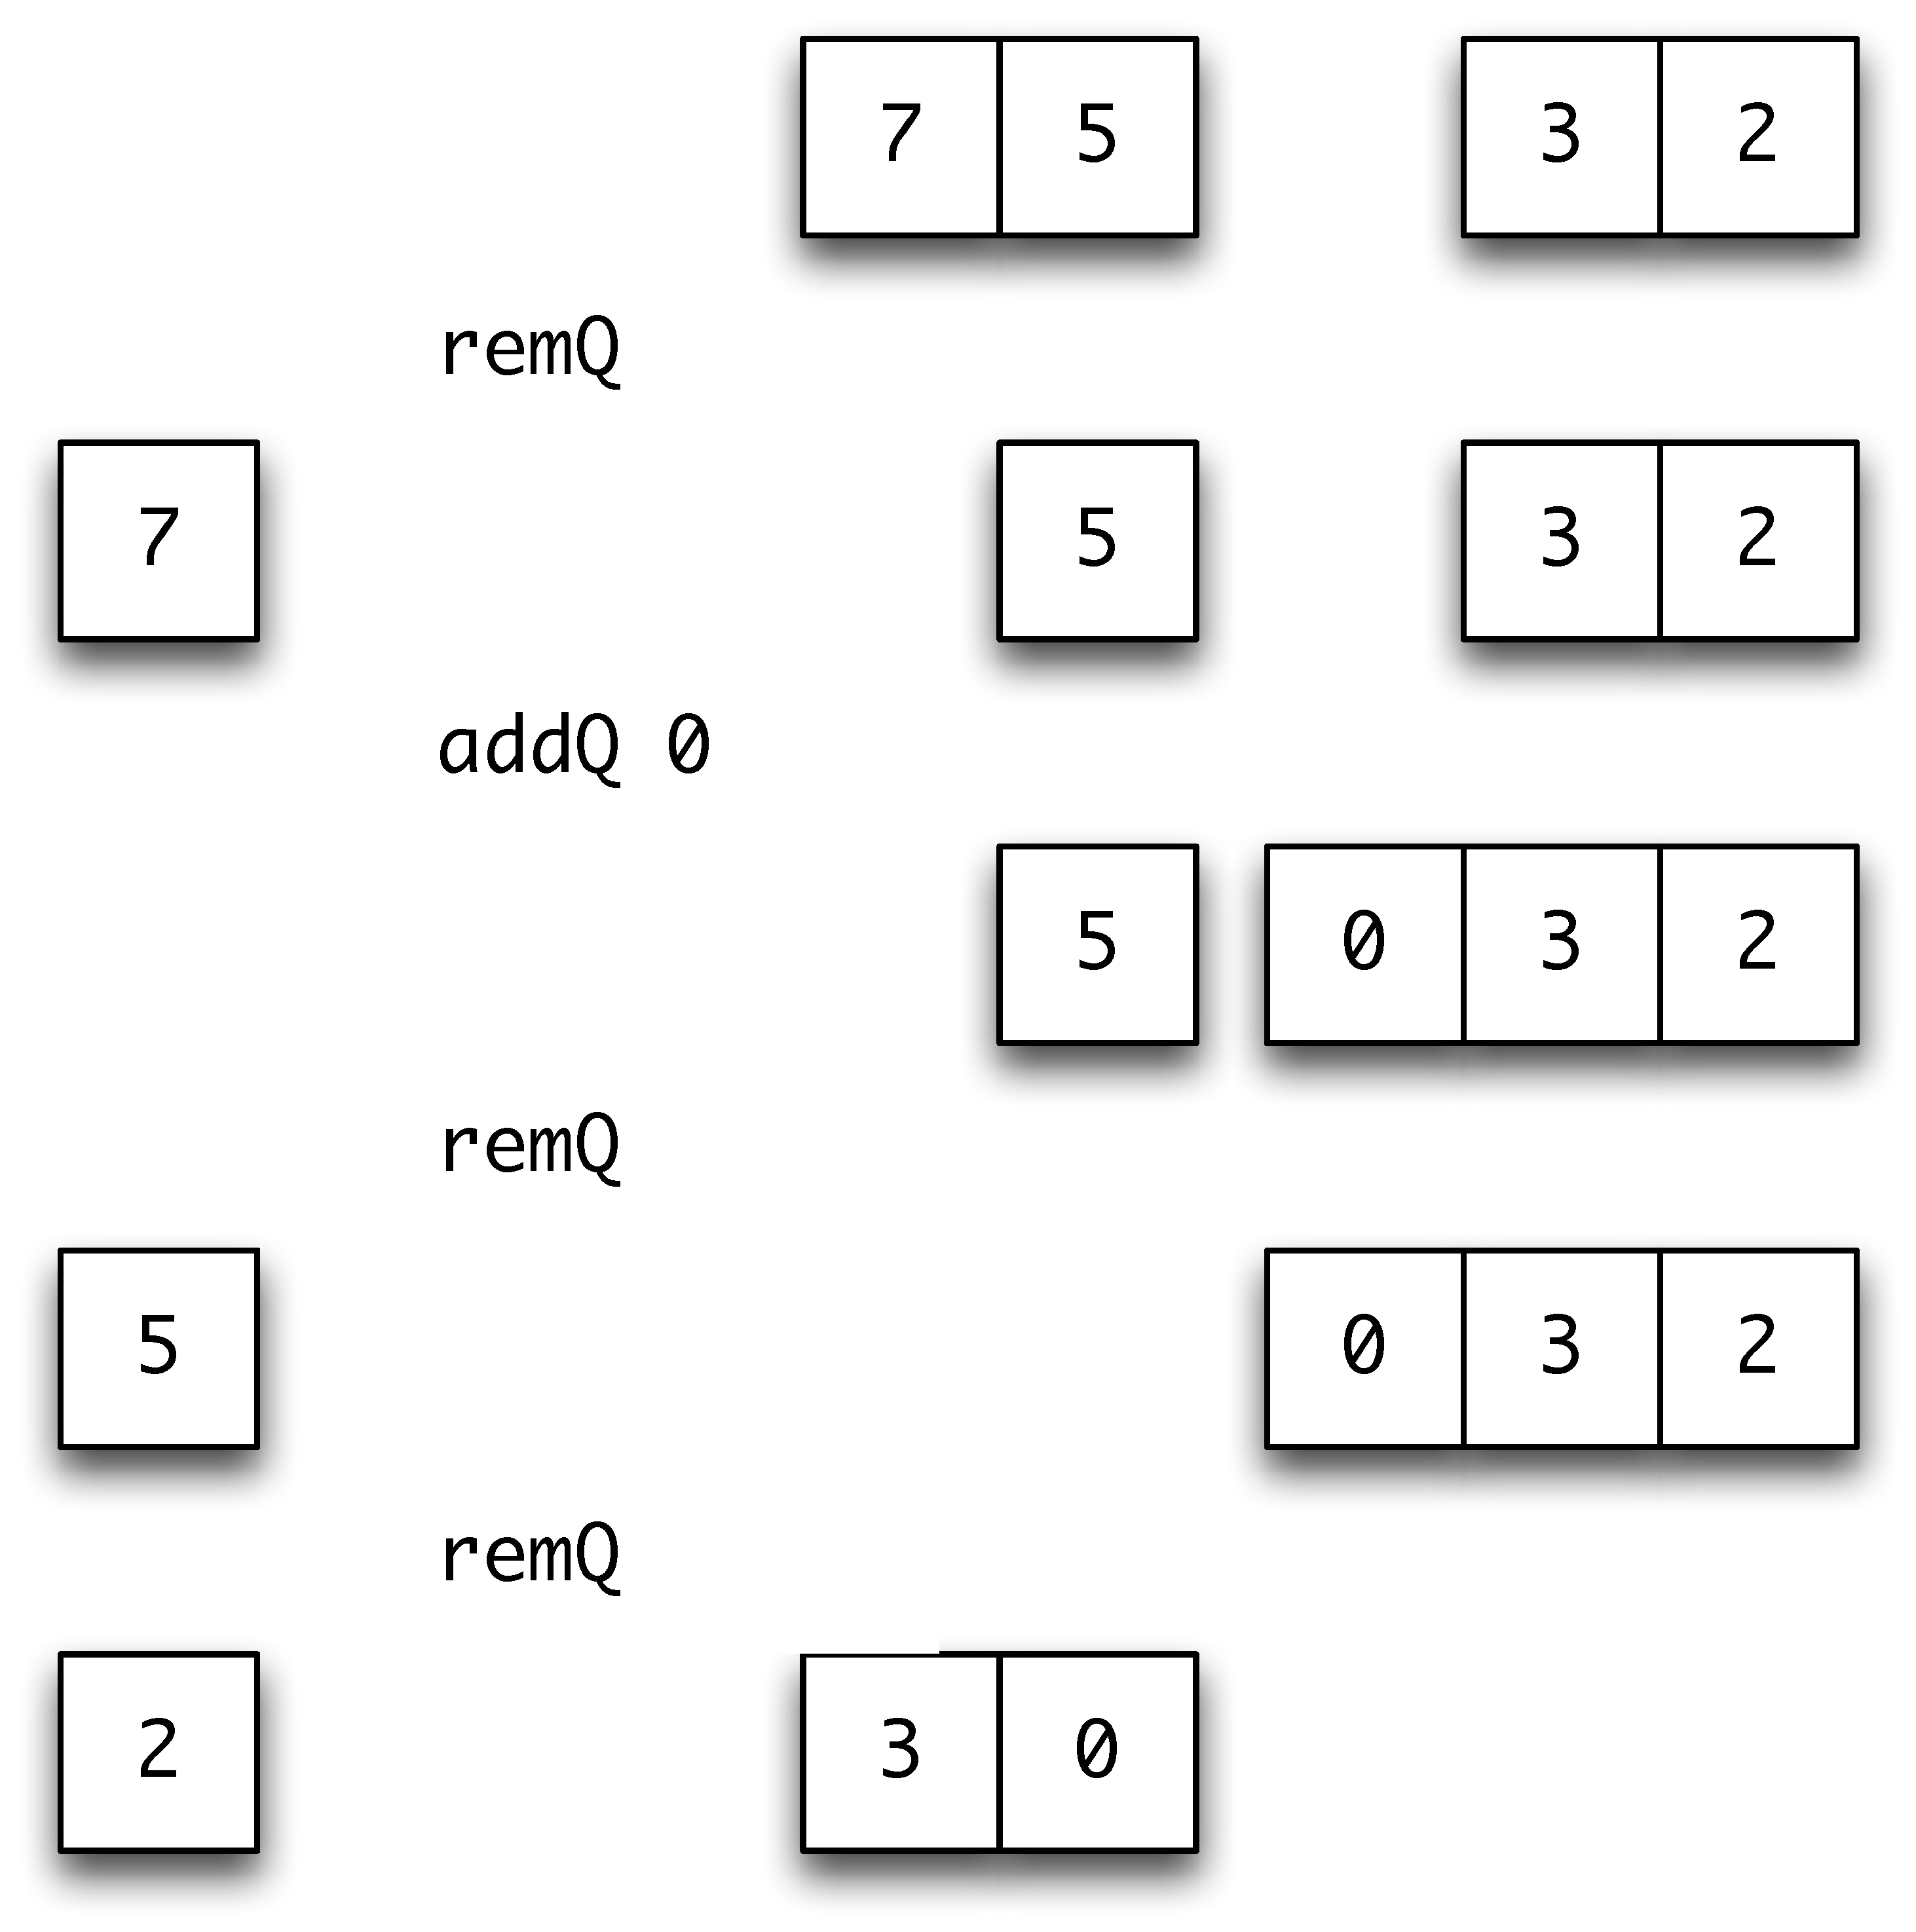
\includegraphics[width=3in]{Pictures/TwoListQueue.pdf}
\end{center}
\begin{alltt}
\end{alltt}
\caption{A two-list queue in action.}
\label{twoListQ}
\end{figure}\index{abstract data type!queue!as two lists}
which represents a number of queues. Initially the queue containing the elements
\texttt{7}, \texttt{5}, \texttt{2} and \texttt{3} is shown: here \texttt{7} is the oldest element in the queue and \texttt{3} the most recent addition. Subsequently
we see the effect of
removing an element, adding the element \texttt{0}, and removing two further
elements. In each case the queue is represented by two lists, each being shown with its head at the left-hand side.

The function \texttt{remQ} removes elements from the head of the left-hand list,
and \texttt{addQ} adds elements to the head of the right. This works until the
left-hand list is empty, when the elements of the right-hand queue have to be
transferred to the
left, reversing their order.  

This case in which we have to transfer elements is expensive, as we have to run
along a list to reverse it,
but we would not in general expect to perform this every
time we remove an element from the queue.
The Haskell implementation follows now.
\begin{alltt}
data Queue a = Queue [a] [a]

emptyQ :: Queue a
emptyQ = Queue [] []

isEmptyQ :: Queue a -> Bool
isEmptyQ (Queue [] []) = True
isEmptyQ _             = False

addQ   :: a -> Queue a -> Queue a
addQ x (Queue xs ys) = Queue xs (x:ys)

remQ   :: Queue a -> (  a , Queue a )
remQ (Queue (x:xs) ys)    = (x , Queue xs ys)
remQ (Queue [] ys@(z:zs)) = remQ (Queue (reverse ys) [])
remQ (Queue [] [])        = error "remQ"
\end{alltt}
As we commented for the \texttt{Store} types, the behaviour of this implementation
will be indistinguishable from the first two, as far as the operations of the
abstract data type
are concerned. On the other hand, the implementation will be
substantially more efficient than the single list implementations, as we
explained above. A thorough examination of recent work on the efficient implementation
of data structures in functional languages  can be found in \citeN{okasakiBook}.
\index{abstract data type!queue|)}

\beware{Using \texttt{newtype}}{
Why didn't we use a \texttt{newtype} in the definition of \texttt{Queue}? The reason is that a  \texttt{newtype} must have a single argument, and \texttt{Queue} has two; we could pair the arguments, and then use a \texttt{newtype}. We leave this as an exercise for the reader.}

\begin{exercises}

\item
Give calculations of
\begin{alltt}
"abcde" ++ "f"
init "abcdef"
last "abcdef"
\end{alltt}
where
\begin{alltt}
init x = take (length x-1) x
last x = x !! (length x-1)
\end{alltt}

\item
Explain the behaviour of the three queue models if you are asked to
perform the following sequence of queue operations: 
add 2,
add 1,
remove item,
add 3,
remove item,
add 1,
add 4,
remove item,
remove item.


\item
Define QuickCheck properties which will test the queue implementations given here. We will show how to define the appropriate generators needed to perform the tests in Chapter \ref{dsls}.


\item
A double-ended queue, or deque, allows elements to be added or removed from
either end of the structure. Give a signature for the ADT \texttt{Deque a},
and give two different implementations of the deque type.

\item
A unique queue can contain only one occurrence of each entry (the one to
arrive earliest). Give a signature for the ADT of these queues, and an
implementation of the ADT.

\item
Each element of a priority queue has a numerical priority. When an element is
removed, it will be of the highest priority in the queue. If there is more
than one of these, the earliest to arrive is chosen. Give a signature and
implementation of the ADT of priority queues. 

\item
{[Harder]}
Examine how priority queues could be used to implement the Huffman coding
system in Chapter \ref{codes}.
\end{exercises}

\section{Design}
\label{adtDesign}
\index{design!abstract data types|(}

This section examines the design of Haskell abstract data types, and how the
presence of this mechanism affects design in general.

\subsection*{General principles}

In building a system, the choice of types is fundamental, and affects the
subsequent design and implementation profoundly. If we use abstract data
types at an early stage we hope to find `natural' representations of the
types occurring in the problem. Designing the abstract data types is a three-stage process.  
\begin{titemize}
\item First we need
to identify and \textbf{name} the types in the system.
\item Next, we should give
an \textbf{informal description} of what is expected from each type. 
\item Using this
description we can then move to writing the \textbf{signature}\index{signature} of each 
abstract data type.
\end{titemize}
How do we decide what should go in the signature? This is the \$64,000
question, of course, but there are some general questions we can ask of any
abstract data type signature.
\begin{titemize}
\item Can we create objects of the type? For instance, in the \texttt{Queue a}
type, we have the object \texttt{emptyQ}, and in a type of sets, we might give a
function taking an element to the `singleton' set containing that element
alone. If there are no such objects or functions, something is wrong!
\item Can we check what sort of object we have? In a tree ADT we might
want to check whether we have a leaf or a node, for instance.
\item Can we extract the components of objects, if we so require? Can we take
the head of a \texttt{Queue a}, say?
\item Can we transform objects: can we reverse a list, perhaps, or add an
item to a queue? 
\item Can we combine objects? We might want to be able to join
together two trees, for example.
\item Can we collapse objects? Can we take the sum of a numerical list, or
find the size of an object, say? 
\end{titemize}
Not all these questions are appropriate in every case, but the majority of
operations we perform on types fall into one of these categories. All the
operations in the following signature for binary trees can be so classified,
for instance.
\begin{alltt}
module Tree\minx{Tree}\index{signature!for \texttt{Tree}}
  (Tree,
   nil,           -- Tree a
   isNil,         -- Tree a -> Bool  
   isNode,        -- Tree a -> Bool
   leftSub,       -- Tree a -> Tree a 
   rightSub,      -- Tree a -> Tree a 
   treeVal,       -- Tree a -> a
   insTree,       -- Ord a => a -> Tree a -> Tree a 
   delete,        -- Ord a => a -> Tree a -> Tree a
   minTree        -- Ord a => Tree a -> Maybe a
  ) where
\end{alltt}
Other functions might be included in the signature; in the case of \texttt{Tree
a} we might want to include the \texttt{size}
function. This function can be defined
using the other operations.
\begin{alltt}
size :: Tree a -> Integer\minx{size}
size t 
  | isNil t     = 0
  | otherwise   = 1 + size (leftSub t) + size (rightSub t)
\end{alltt}
This definition of \texttt{size} is \textbf{independent} of the implementation,
and so would not have to be reimplemented if the implementation type for
\texttt{Tree a} changed. This is a good reason for leaving \texttt{size} out
of the signature, and this is a check we can make for any signature: are all
the functions in the signature needed? We come back to this point, and the
tree type, later in the chapter. Now we look at a larger-scale example.

\begin{exercises}

\item
Are all the operations in the \texttt{Tree a} signature necessary? Identify those
which can be implemented using the other operations of the signature.

\item
Design a signature for an abstract type of library databases, as first
introduced in Chapter \ref{tupleList}.

\item
Design a signature for an abstract type of indexes, as examined in Section
\ref{indexExam}. 

\index{abstract data type|)}
\index{design!abstract data types|)}
\end{exercises}
\section{Simulation}
\index{simulation|(}

\label{simEx}

We first introduced the simulation example in Section \ref{algDesign}, where
we designed the algebraic types \texttt{Inmess} and \texttt{Outmess}. Let us
suppose, for ease of exposition, that the system time is measured in minutes.

The \minx{Inmess}\minx{Outmess}
\texttt{Inmess} \texttt{No} signals no arrival, while \texttt{Yes 34 12} signals the
arrival of a customer at the \texttt{34}th minute, who will need \texttt{12} minutes
to be served. 

The \texttt{Outmess} \texttt{Discharge 34 27 12} signals that the person arriving
at time \texttt{34} waited \texttt{27} minutes before receiving their \texttt{12}
minutes of service.

Our aim in this section is to design the ADTs for a simple
simulation of queueing. We start by looking at a single queue. Working
through the stages, we will call the type \texttt{QueueState}, and it can be
described thus. 
\begin{quote}
There are two main operations on a queue. The first is to add a new item, an
\texttt{Inmess}, to the queue. The second is to process the queue by a one-minute
step; the effect of this is to give one minute's further processing to the
item at the head of the queue (if there is such a thing). Two outcomes are
possible: the item might have its processing completed, in which case an 
\texttt{Outmess} is generated, or further processing may be needed.

Other items we need are an empty queue, an indication of
the length of a queue and a test of whether a queue is empty.
\end{quote}
This description leads directly to a signature declaration
\begin{alltt}
module QueueState \minx{QueueState}
  ( QueueState ,
    addMessage,      -- Inmess -> QueueState -> QueueState
    queueStep,       -- QueueState -> ( QueueState , [Outmess] )
    queueStart,      -- QueueState
    queueLength,     -- QueueState -> Int
    queueEmpty       -- QueueState -> Bool
    ) where
\end{alltt}
The \texttt{queueStep} function returns a pair: the \texttt{QueueState}
after a step of
processing, and a \textbf{list} of \texttt{Outmess}. A list is used, rather
than a single \texttt{Outmess}, so that in the case of no output an empty list
can be returned.

The \texttt{QueueState} type allows us to model a situation in which all
customers are served by a single processor (or bank clerk). How can we model
the case where there is more than one queue? We call this a \textbf{server}
and it is to be modelled by the \texttt{ServerState} ADT.
\begin{quote}
A server consists of a collection of queues, which can be identified by
the integers \texttt{0}, \texttt{1} and so on. It is assumed that the system
receives one \texttt{Inmess} each minute: at most one person arrives every
minute, in other words. 
 
There are three principal operations on a server.
First, we should be able to add an \texttt{Inmess} to one of the queues.
Second, a processing step of the server is given by processing each of the
constituent queues by one step: this can generate a list of \texttt{Outmess}, as
each queue can generate such a message. Finally, a step of the simulation
combines a server step with allocation of the \texttt{Inmess} to the shortest
queue in the server.

Three other operations are necessary. We have a starting server, consisting
of the appropriate number of empty queues, and we should be able to identify
the number of queues in a server, as well as the shortest queue it contains.

\end{quote}
\vspace{5pt}

As a signature, we have
\begin{alltt}
module ServerState \minx{ServerState}
  ( ServerState ,
    addToQueue,     -- Int -> Inmess -> ServerState -> ServerState
    serverStep,     -- ServerState -> ( ServerState , [Outmess] )
    simulationStep, -- ServerState -> Inmess -> ( ServerState , 
                                                  [Outmess] ) 
    serverStart,    -- ServerState
    serverSize,     -- ServerState -> Int
    shortestQueue   -- ServerState -> Int
  ) where
\end{alltt}
In the next section we explore how to implement these two abstract data types.
It is important to realize that users of the ADTs can begin to do their
programming now: all the information that they need to know is contained
in the signature of the abstract data type.\looseness=-1

\begin{exercises}
\item
Are there redundant operations in the signatures of the ADTs 
\texttt{QueueState} and \texttt{ServerState}?

\item
Design a signature for \textbf{round-robin} simulation,
in which allocation of the first item is to queue \texttt{0}, the second to queue
\texttt{1}, and so on, starting again at \texttt{0} after the final queue has had an 
element assigned to it. 
\end{exercises}

\section{Implementing the simulation}

This section gives an implementation of the ADTs for a queue and a
server. The \texttt{QueueState} is implemented from scratch, while the 
\texttt{ServerState} implementation builds on the \texttt{QueueState} ADT. This
means that the two implementations are independent; modifying the
implementation of \texttt{QueueState} has no effect on the implementation of
\texttt{ServerState}.
\subsection*{The queue}
\index{simulation!the queue}

In the previous section, we designed the interfaces for the ADT;
how do we proceed with implementation? First we ought to look again at the
description of the \texttt{QueueState} type. What information does this imply
the type should contain?
\begin{titemize}
\item There has to be a \textbf{queue} of \texttt{Inmess} to be processed. This
can be represented by a list, and we can take the item at the head of the
list as the item currently being processed.
\item We need to keep a record of the processing time given to the head item,
up to the particular time represented by the state.
\item In an \texttt{Outmess}, we need to give the waiting
time for the particular item being processed. We know the time of arrival
and the time needed for processing -- if we also know the current time, we
can calculate the waiting time from these three numbers.
\end{titemize} 
It therefore seems sensible to define
\begin{alltt}
data QueueState = QS Time Service [Inmess]
                  deriving (Eq, Show)\minx{QueueState}
\end{alltt}
where the first field gives the current time, the second the service time so
far for the item currently being processed,
and the third the queue itself. Now we look at the operations one by one.
To add a message, it is put at the end of the list of messages.
\begin{alltt}
addMessage  :: Inmess -> QueueState -> QueueState

addMessage im (QS time serv ml) = QS time serv (ml++[im])
\end{alltt}
The most complicated definition is of \texttt{queueStep}. As was explained
informally, there are two principal cases, when there is an item being
processed.
\begin{alltt}
queueStep   :: QueueState -> ( QueueState , [Outmess] )\minx{queueStep}

queueStep (QS time servSoFar (Yes arr serv : inRest))
  | servSoFar < serv
    = (QS (time+1) (servSoFar+1) (Yes arr serv : inRest) , [])
  | otherwise
    = (QS (time+1) 0 inRest , [Discharge arr (time-serv-arr) serv])
\end{alltt}
In the first case, when the service time so far (\texttt{servSoFar}) is smaller
than is required (\texttt{serv}), processing is not complete. We therefore add one to
the time, and the service so far, and produce no output message. 
 
If processing is complete -- which is the
\texttt{otherwise} case -- the new state of the queue is  
\texttt{QS (time+1) 0 inRest}. In this state the time is advanced by one,  
processing time is set to zero and the head item in the list is removed.
An output message is also produced in which the
waiting time is given by subtracting the service and arrival times from the
current time.

If there is nothing to process, then we simply have to advance the current
time by one, and produce no output.
\begin{alltt}
queueStep (QS time serv []) = (QS (time+1) serv [] , [])
\end{alltt}
Note that the case of an input message \texttt{No} is not handled here since these
messages
are filtered out by the server; this is discussed below.

The three other functions are given by
\begin{alltt}
queueStart  :: QueueState
queueStart  =  QS 0 0 [] 

queueLength :: QueueState -> Int
queueLength (QS _ _ q) = length q

queueEmpty  :: QueueState -> Bool
queueEmpty (QS _ _ q)  = (q==[])
\end{alltt}
and this completes the implementation.

Obviously there are different possible implementations. We might choose to
take the item being processed and hold it separately from the queue, or
to use an ADT for the queue part, rather than a `concrete' list. 

\subsection*{The server}
\index{simulation!the server}

The server consists of a collection of queues, accessed by integers from 
\texttt{0}; we choose to use a \textbf{list} of queues.
\begin{alltt}
newtype ServerState = SS [QueueState] 
                         deriving (Eq, Show)\minx{ServerState}
\end{alltt}
Note that the implementation of this ADT builds on another ADT; this
is not unusual. Now we take the functions in turn.

Adding an element to a queue uses the function \texttt{addMessage} from the 
\texttt{QueueState} abstract type.
\begin{alltt}\minx{addToQueue} 
addToQueue :: Int -> Inmess -> ServerState -> ServerState
 
addToQueue n im (SS st)
  = SS (take n st ++ [newQueueState] ++ drop (n+1) st)
    where
    newQueueState = addMessage im (st!!n)
\end{alltt}
A step of the server is given by making a step in each of the constituent
queues, and concatenating together the output messages they produce.
\begin{alltt} 
serverStep :: ServerState -> ( ServerState , [Outmess] )\minx{serverStep}

serverStep (SS [])
  = (SS [],[])
serverStep (SS (q:qs)) 
  =  (SS (q':qs') , mess++messes)
    where
    (q' , mess)       = queueStep  q
    (SS qs' , messes) = serverStep (SS qs)
\end{alltt}
In making a simulation step, we perform a server step, and then add the
incoming message, if it indicates an arrival, to the shortest queue. 
\begin{alltt}
simulationStep       \minx{simulationStep}
  :: ServerState -> Inmess -> ( ServerState , [Outmess] )

simulationStep servSt im 
  = (addNewObject im servSt1 , outmess)
    where
    (servSt1 , outmess) = serverStep servSt
\end{alltt}
Adding the message to the shortest queue is done by \texttt{addNewObject}, which
is not in the signature. The reason for this is that it can be defined using
the operations \texttt{addToQueue} and \texttt{shortestQueue}.
\begin{alltt}
addNewObject :: Inmess -> ServerState -> ServerState

addNewObject No servSt = servSt

addNewObject (Yes arr wait) servSt
  = addToQueue (shortestQueue servSt) (Yes arr wait) servSt
\end{alltt}
It is in this function that the input messages \texttt{No} are not passed to the
queues, as was mentioned above.

The other three functions of the signature are standard.
\begin{alltt}
serverStart :: ServerState
serverStart = SS (replicate numQueues queueStart) 
\end{alltt}
where \texttt{numQueues} is a constant to be defined, and the standard function
\texttt{replicate} returns a list of \texttt{n} copies of \texttt{x} when applied thus: 
\texttt{replicate n x}.
\begin{alltt} 
serverSize :: ServerState -> Int
serverSize (SS xs) = length xs
\end{alltt}
In finding the shortest queue, we use the \texttt{queueLength} function from the
\texttt{QueueState} type.
\begin{alltt}
shortestQueue :: ServerState -> Int
 
shortestQueue (SS [q]) = 0
shortestQueue (SS (q:qs)) 
  | (queueLength (qs!!short) <= queueLength q)   = short+1
  | otherwise                                    = 0
      where
      short = shortestQueue (SS qs)
\end{alltt}
This concludes the implementation of the two simulation ADTs. The example
is intended to show the merit of designing in stages. First we gave an
informal description of  the operations on the types, then a description of
their signature, and finally an implementation. Dividing the problem up in
this way makes each stage easier to solve. 

The example also shows that types
can be implemented \textbf{independently}: since \texttt{ServerState} uses only the
abstract data type operations over \texttt{QueueState}, we can reimplement  
\texttt{QueueState} without affecting the server state at all.

\begin{exercises} 

\item
Give calculations of the expressions
\begin{alltt}
queueStep (QS 12 3 [Yes 8 4])
queueStep (QS 13 4 [Yes 8 4])
queueStep (QS 14 0 [])
\end{alltt}

\item
If we let
\begin{alltt}
serverSt1 = SS [ (QS 13 4 [Yes 8 4]) , (QS 13 3 [Yes 8 4]) ]
\end{alltt}
then give calculations of 
\begin{alltt}
serverStep serverSt1
simulationStep (Yes 13 10) serverSt1
\end{alltt}


\item
Define QuickCheck properties which will test the simulation system. We will show how to define the appropriate generators needed to perform the tests in Chapter \ref{dsls}.



\item
Explain why we cannot use the function type \texttt{(Int -> QueueState)} as the
representation type of \texttt{ServerState}. Design an extension of this type
which will represent the server state, and implement the functions of the
signature over this type.

\item
Given the implementations of the ADTs from this section,
is your answer to the question of
whether there are redundant operations in the signatures of queues and servers
any different?

\item
If you have not done so already, design a signature for round-robin simulation,
in which allocation of the first item is to queue \texttt{0}, the second to queue
\texttt{1}, and so on. 

\item 
Give an implementation of the round-robin simulation which {\em uses\/} the 
\texttt{ServerState} ADT.

\item
Give a different implementation
of the round-robin simulation which {\em modifies\/}
the implementation of the type \texttt{ServerState} itself.
\end{exercises}
\index{simulation|)}


\section{Search trees}
\label{srchTrees}
\index{search tree|(}

A binary search tree is an object of type \texttt{Tree a} whose elements are
\textbf{ordered}.  A general binary tree is implemented by the algebraic
data type \texttt{Tree}:
\begin{alltt}\minx{Tree}
data Tree a = Nil | Node a (Tree a) (Tree a)
\end{alltt}
When is a tree ordered?
The tree {\mi(Node val \tone\ \ttwo)} is ordered if 
\begin{titemize}
\item all values in \texttt{\tone} are
smaller than \texttt{val},  
\item all values in \texttt{\ttwo} are larger than \texttt{val}, and
\item the trees \texttt{\tone} and \texttt{\ttwo} are themselves ordered;
\end{titemize}
and the tree \texttt{Nil} is ordered.

Search trees are used to represent sets of elements, for instance. How can we
create a type of search trees? The concrete (algebraic) type \texttt{Tree a} will not serve, as it
contains elements like \texttt{Node 2 (Node 3 Nil Nil) Nil}, which are not
ordered.

The answer is to build elements of the type \texttt{Tree a}
using only operations which create
or preserve order. We ensure that only these `approved' operations are used
by making the type an abstract data type. 

\subsection*{The abstract data type for search trees}
\index{abstract data type!search tree}

We discussed the signature of the abstract data type earlier, in Section
\ref{adtDesign}, but we repeat it here.
\begin{alltt}
module Tree\minx{Tree}\index{signature!for \texttt{Tree}}
  (Tree,
   nil,           -- Tree a
   isNil,         -- Tree a -> Bool  
   isNode,        -- Tree a -> Bool
   leftSub,       -- Tree a -> Tree a 
   rightSub,      -- Tree a -> Tree a 
   treeVal,       -- Tree a -> a
   insTree,       -- Ord a => a -> Tree a -> Tree a 
   delete,        -- Ord a => a -> Tree a -> Tree a
   minTree        -- Ord a => Tree a -> Maybe a
  ) where
\end{alltt}
As we have said, the
implementation type is 
\begin{alltt}
data Tree a = Nil | Node a (Tree a) (Tree a)\minx{Tree}
\end{alltt}
and the standard operations to discriminate between different sorts of
tree and to extract components are defined by
\begin{alltt}
nil :: Tree a\minx{nil}
nil = Nil

isNil :: Tree a -> Bool\minx{isNil}
isNil Nil = True
isNil _   = False

isNode :: Tree a -> Bool\minx{isNode}
isNode Nil = False 
isNode _   = True

leftSub :: Tree a -> Tree a\minx{leftSub}
leftSub Nil            = error "leftSub"
leftSub (Node _ t1 _)  = t1

rightSub :: Tree a -> Tree a\minx{rightSub}
rightSub Nil            = error "rightSub"
rightSub (Node _ _ t2)  = t2

treeVal  :: Tree a -> a\minx{treeVal}
treeVal Nil            = error "treeVal"
treeVal (Node v _ _)   = v
\end{alltt}

\begin{figure}[t]
\begin{center}
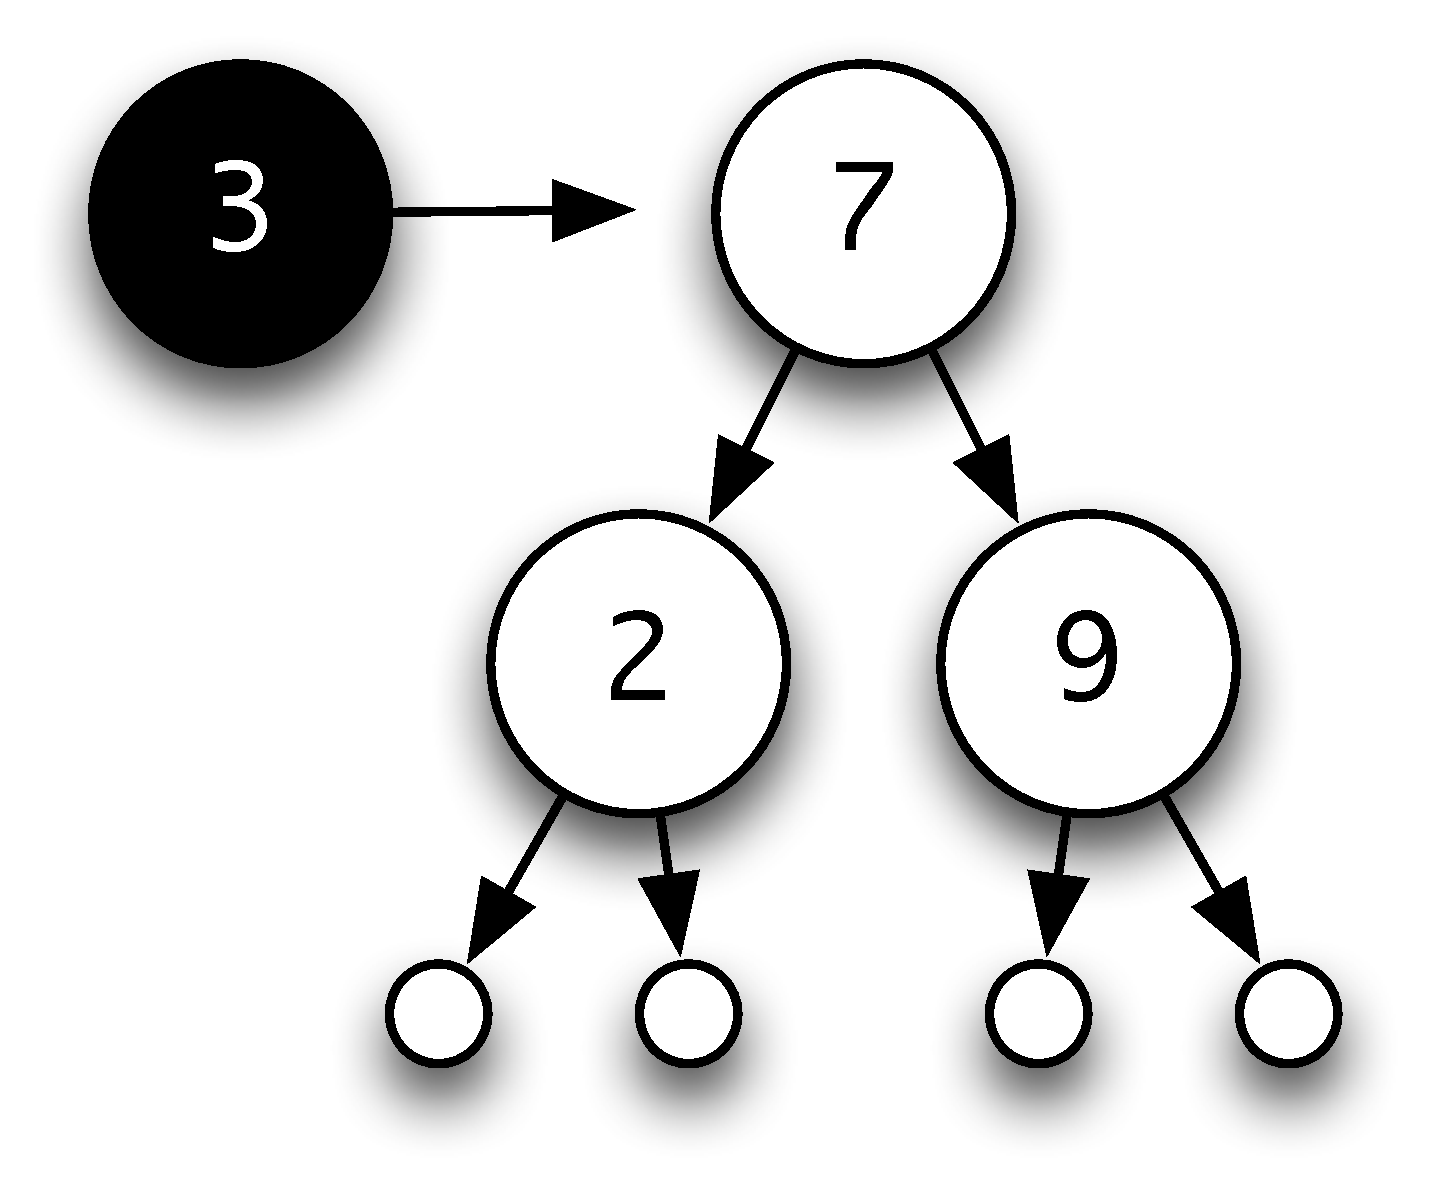
\includegraphics[width=1.3in]{Pictures/SearchTree1.pdf}\hfill
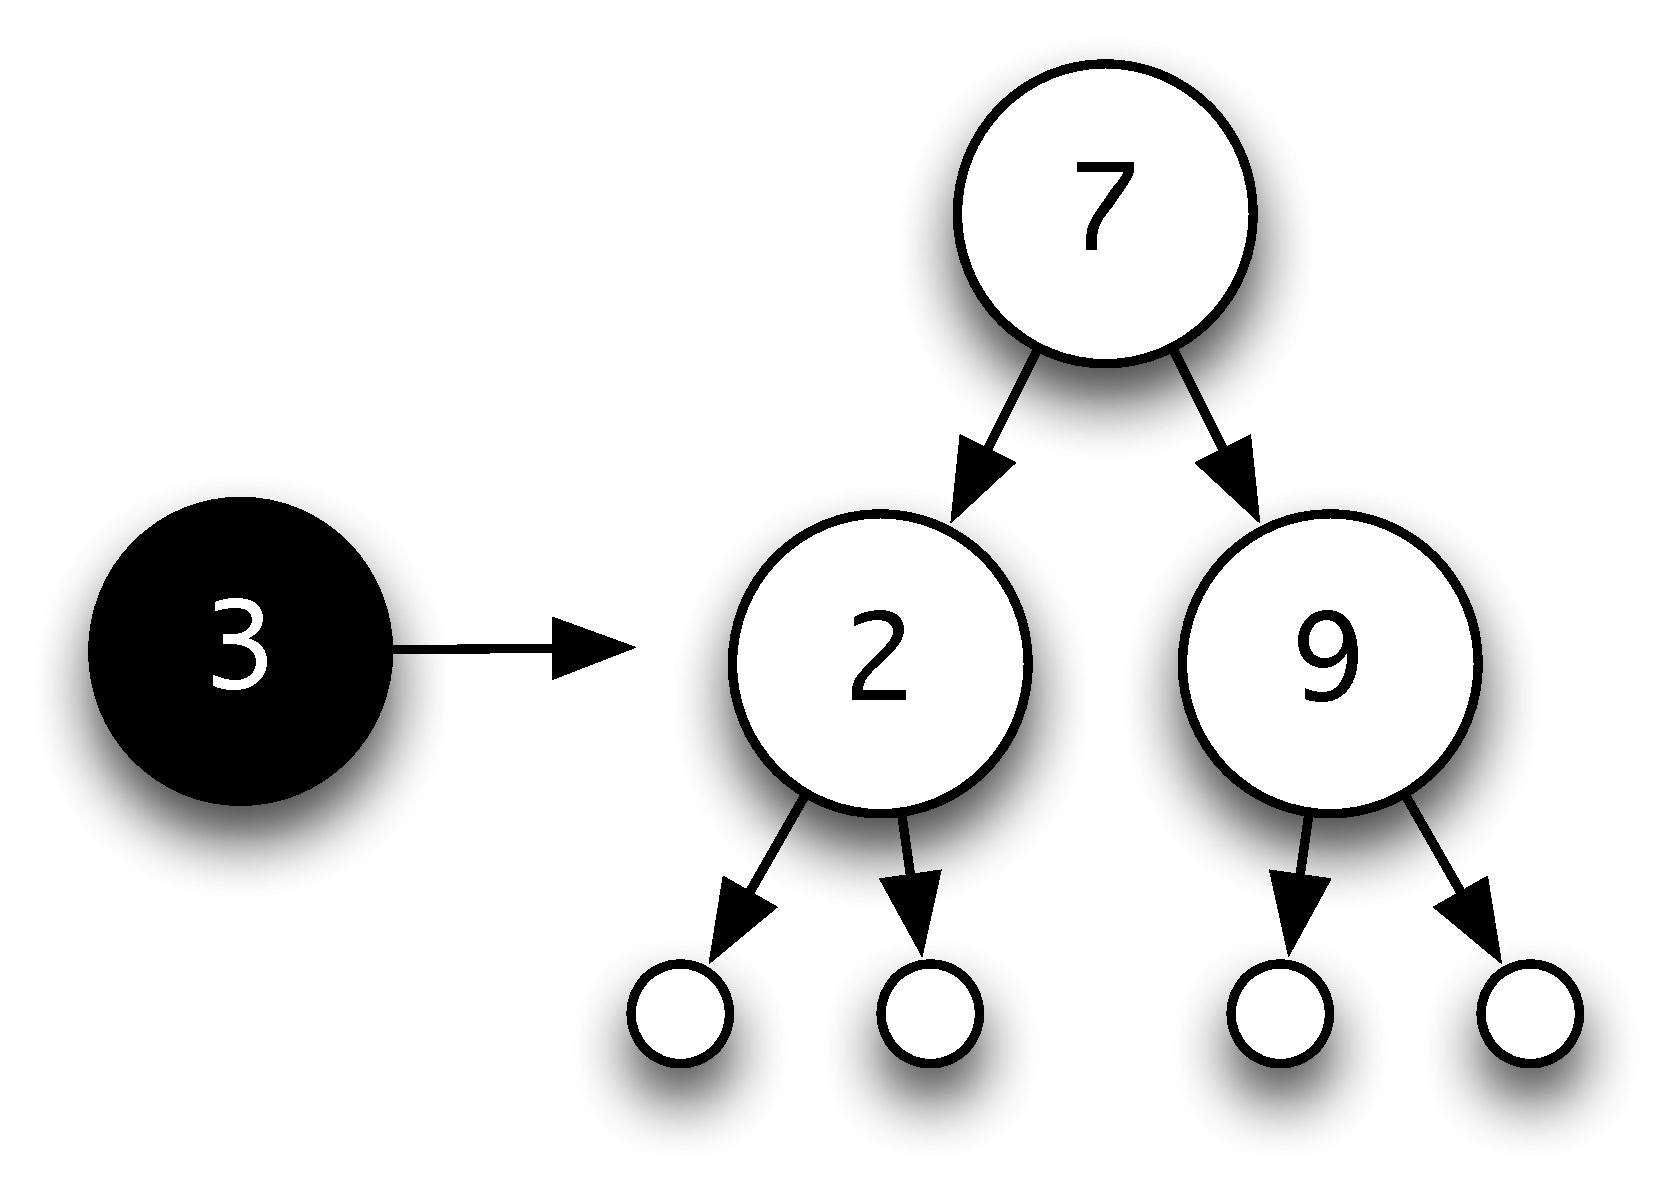
\includegraphics[width=1.5in]{Pictures/SearchTree2.pdf}\hfill
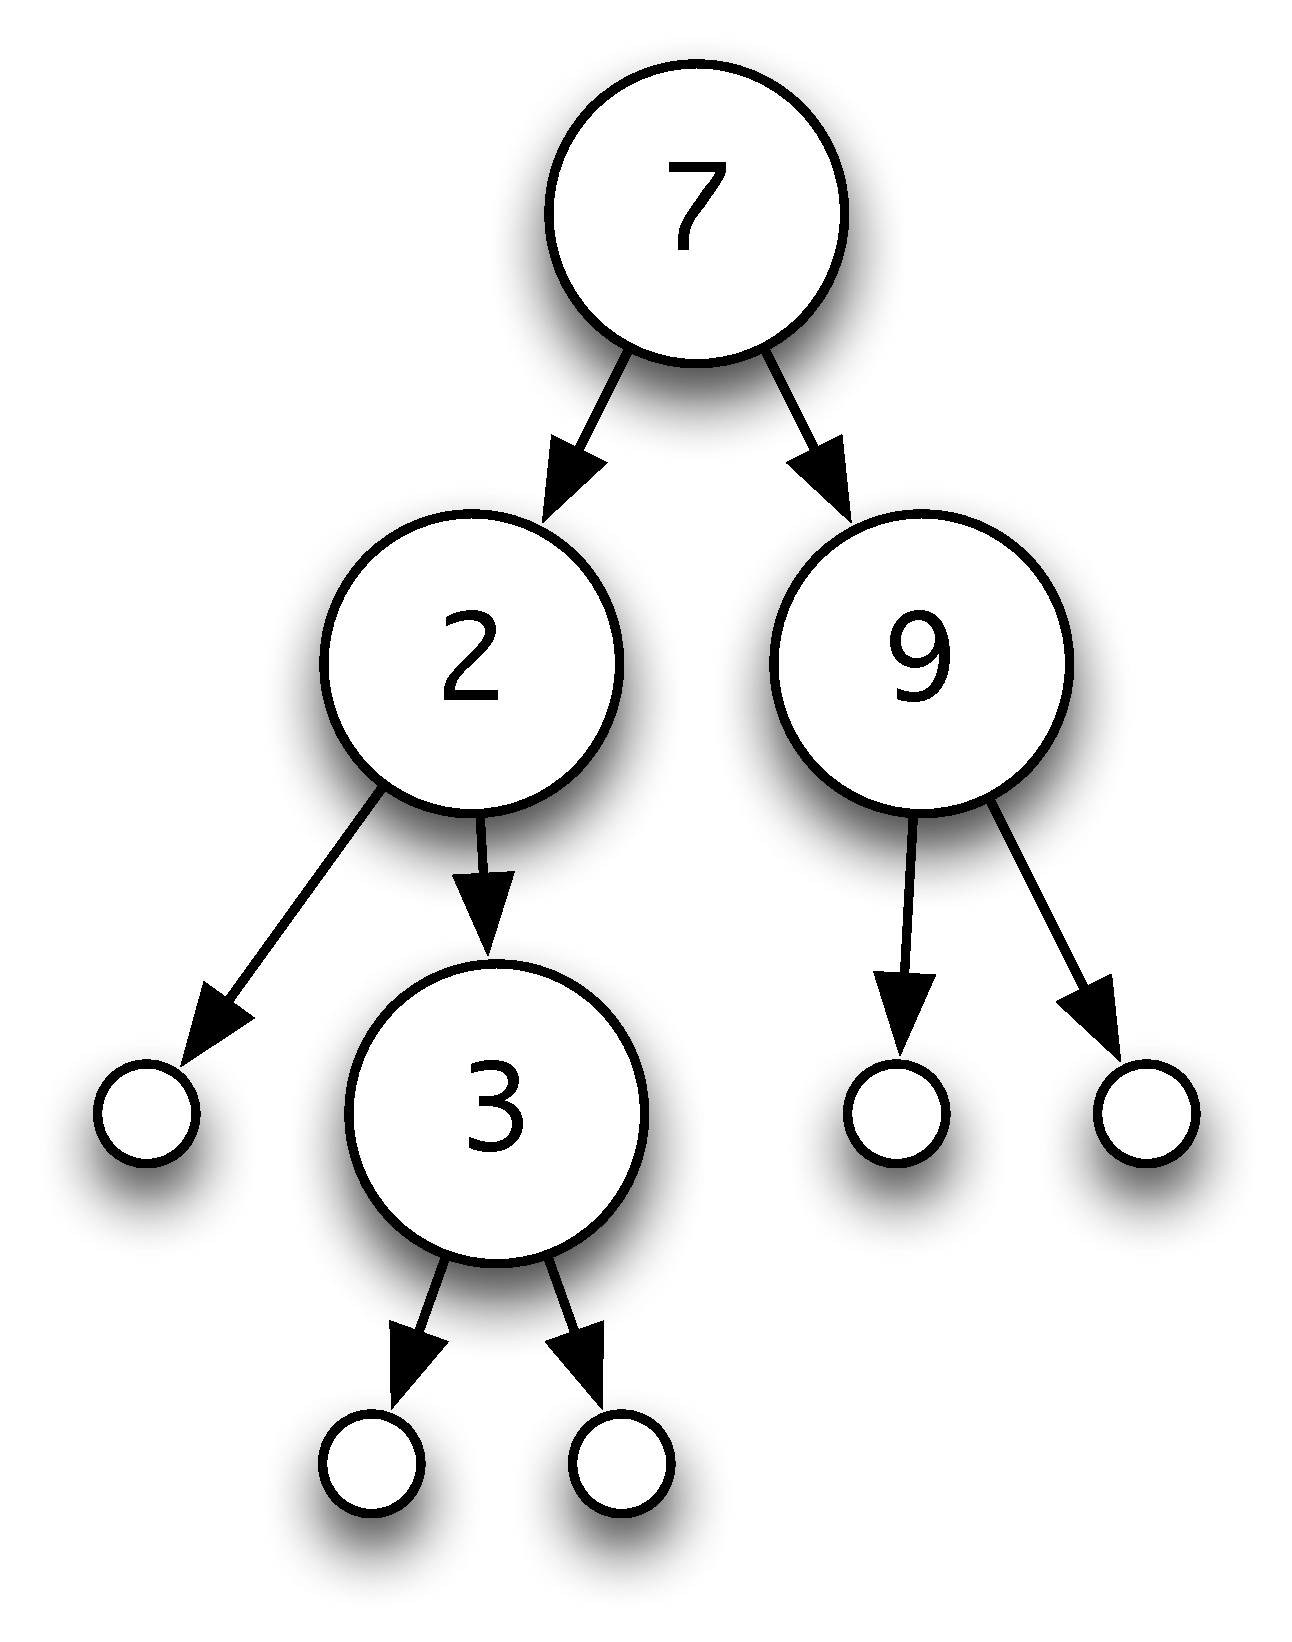
\includegraphics[width=1.2in]{Pictures/SearchTree3.pdf}
\end{center}
\caption{Insertion into a search tree}
\label{insertSearchTree}
\end{figure}



\begin{figure}
\begin{alltt}
insTree :: Ord a => a -> Tree a -> Tree a\minx{insTree}

insTree val Nil = (Node val Nil Nil)

insTree val (Node v t1 t2)
  | v==val      = Node v t1 t2
  | val > v     = Node v t1 (insTree val t2)	
  | val < v     = Node v (insTree val t1) t2	

delete :: Ord a => a -> Tree a -> Tree a\minx{delete}

delete val (Node v t1 t2)
  | val < v     = Node v (delete val t1) t2
  | val > v     = Node v t1 (delete val t2)
  | isNil t2    = t1
  | isNil t1    = t2
  | otherwise   = join t1 t2

minTree :: Ord a => Tree a -> Maybe a\minx{minTree}

minTree t
  | isNil t     = Nothing
  | isNil t1    = Just v
  | otherwise   = minTree t1
      where
      t1 = leftSub t
      v  = treeVal t

--      join is an auxiliary function, used in delete;
--      it is not exported.

join :: Ord a => Tree a -> Tree a -> Tree a\minx{join}

join t1 t2 
  = Node mini t1 newt
    where
    (Just mini) = minTree t2
    newt        = delete mini t2 
\end{alltt}
\caption{Operations over search trees.}
\label{treeOps}
\index{search tree!operations}
\end{figure}
\noindent
Figure \ref{treeOps} contains the definitions of the insertion, deletion and
\index{search tree!insertion}
join functions. The function \texttt{join} is used
to join two trees with the property that all elements in the left are
smaller than all in the right; that will be the case for the call in
\texttt{delete} where it is used. It is not exported, as it can break the ordered property of
search trees if it is applied to an arbitrary pair of search trees.

\begin{figure}[t]
\begin{center}
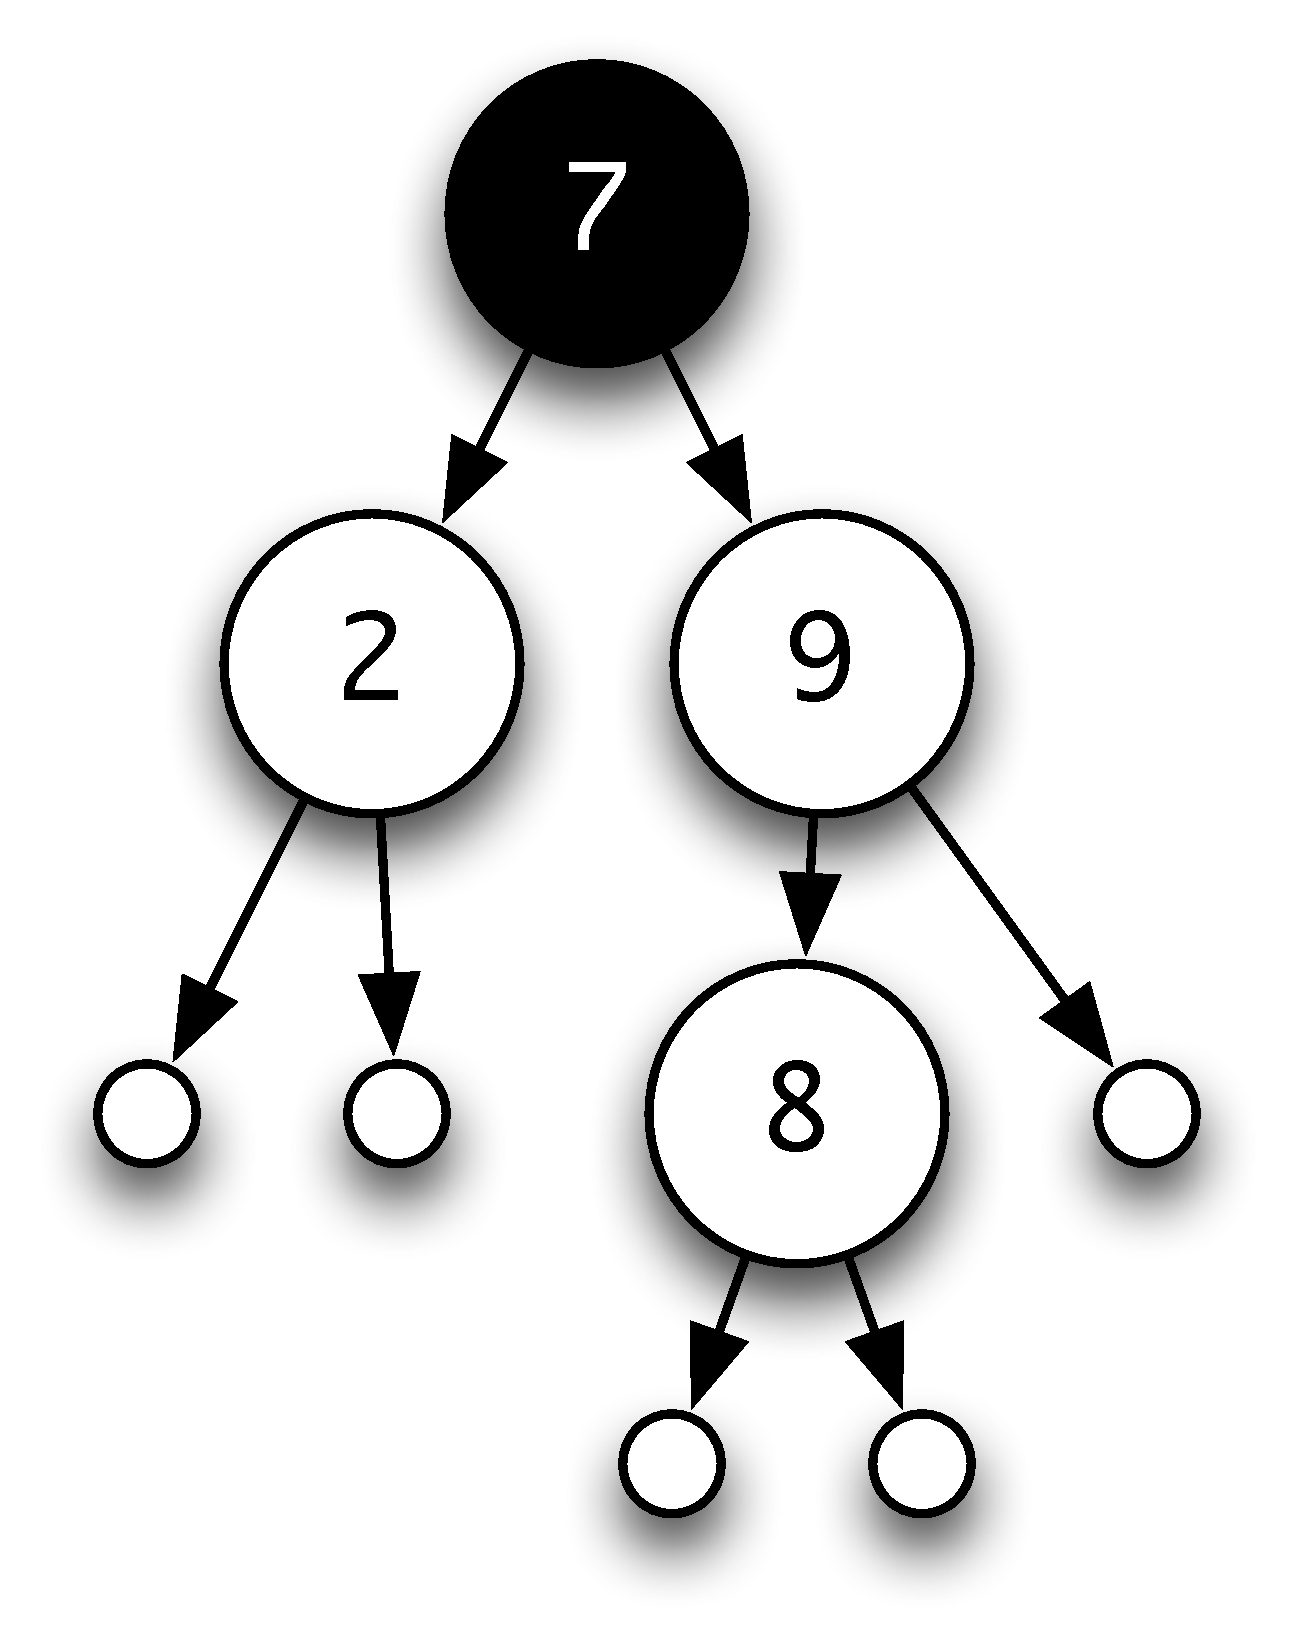
\includegraphics[width=1.1in]{Pictures/SearchTree4.pdf}\hfill
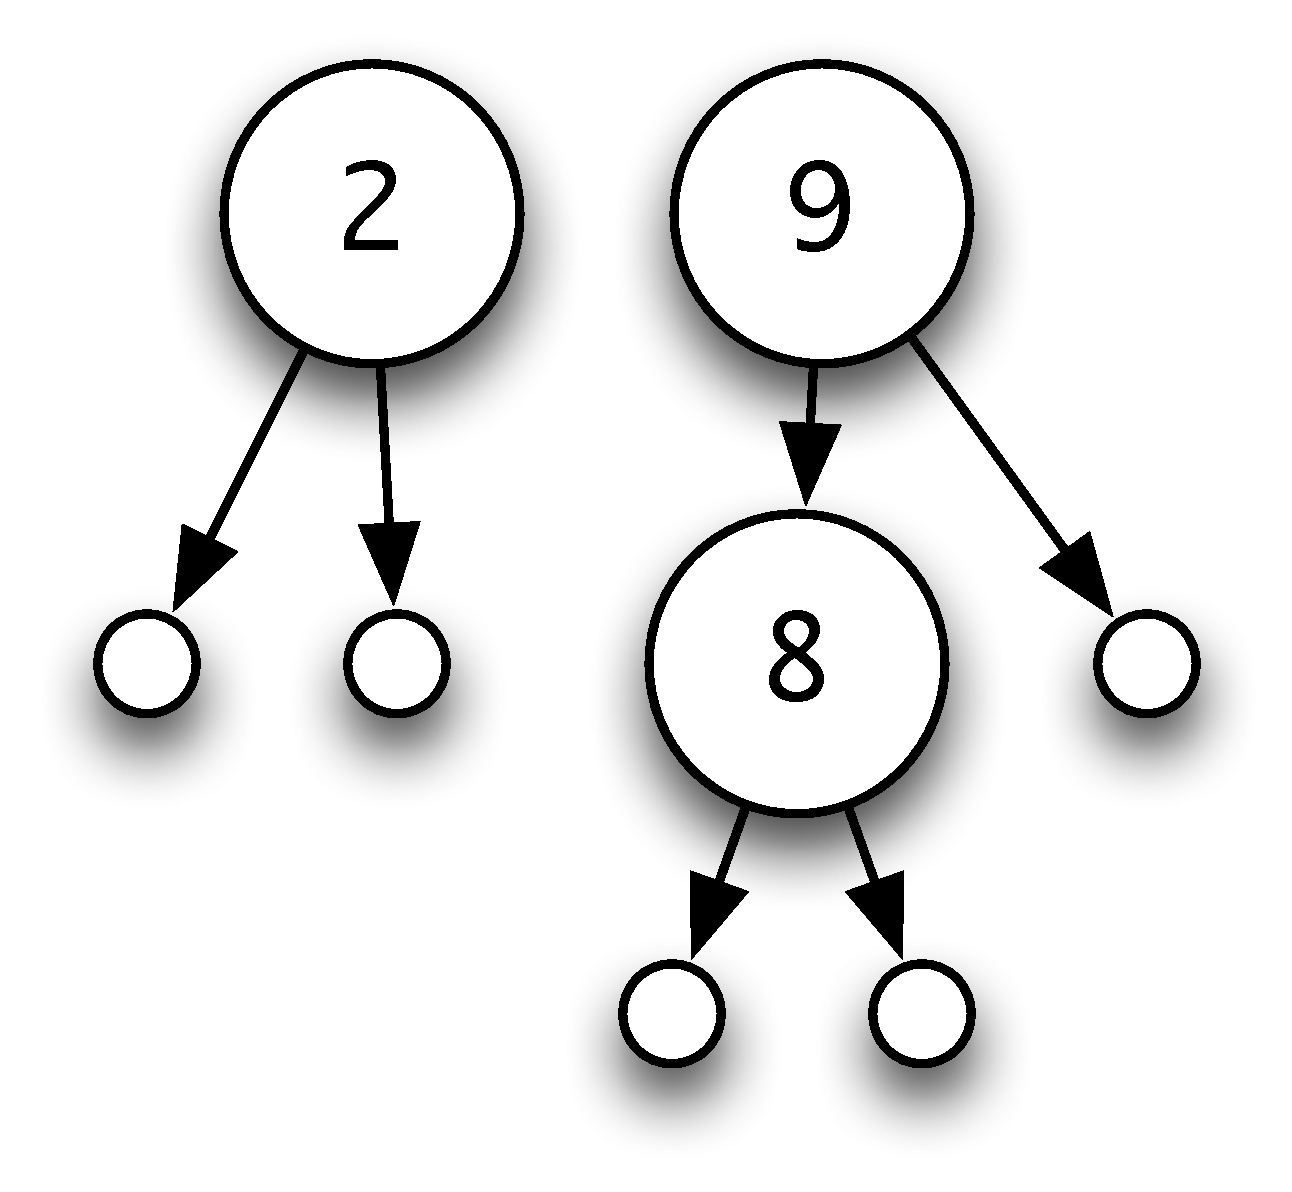
\includegraphics[width=1.1in]{Pictures/SearchTree5.pdf}\hfill
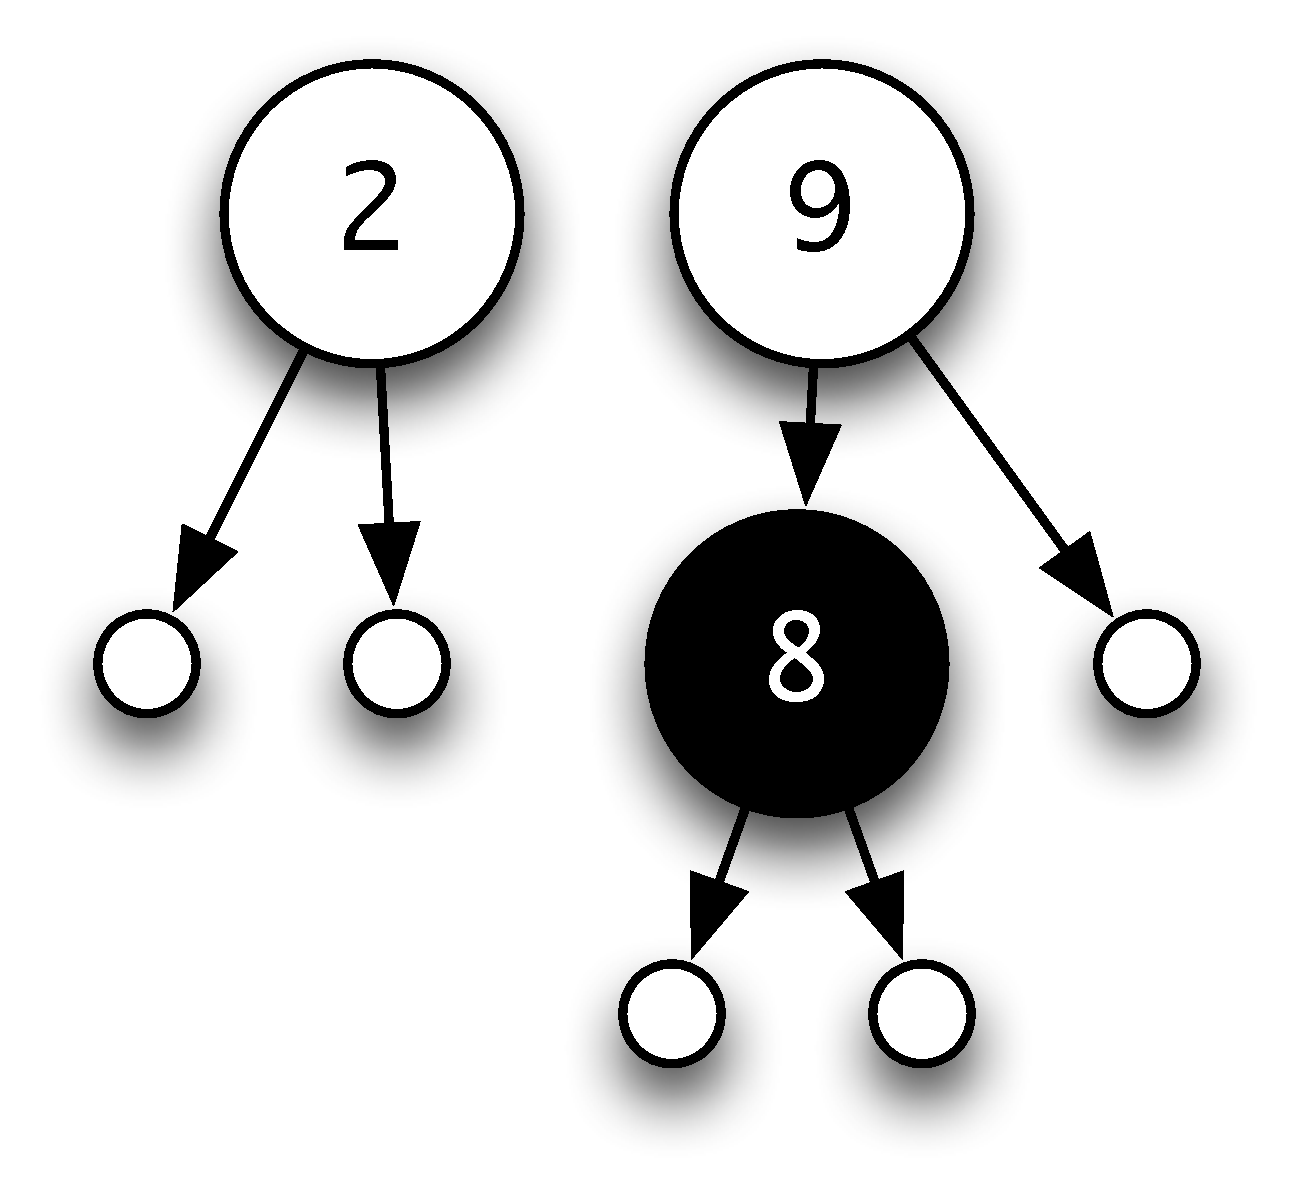
\includegraphics[width=1.1in]{Pictures/SearchTree6.pdf}\hfill
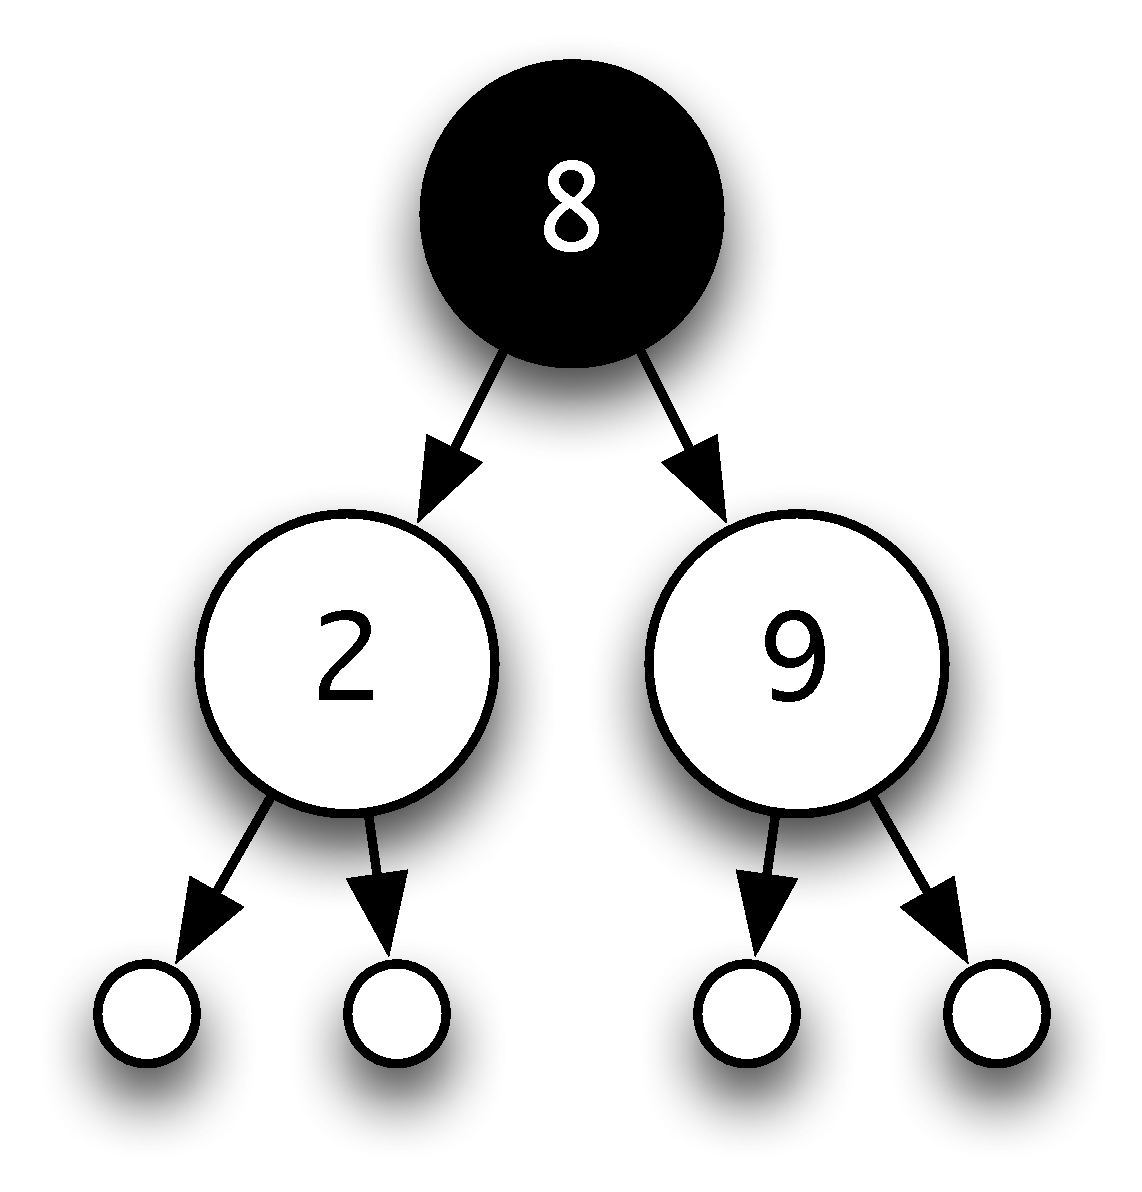
\includegraphics[width=1in]{Pictures/SearchTree7.pdf}
\end{center}
\caption{Deletion from a search tree}
\label{deleteSearchTree}
\end{figure}




Note that the types of \texttt{insTree}, \texttt{delete},
\texttt{minTree} and \texttt{join}
contain the
context \texttt{Ord a}.\minx{Ord}
Recall from Chapter \ref{classes} that this constraint means that
these functions can only be used over types which carry an ordering operation,
\texttt{<=}. It is easy to see from the definitions of these functions that they
do indeed use the ordering, and given the definition of search trees it
is unsurprising that we use an ordering in these operations. Now we look
at the definitions in Figure \ref{treeOps} in turn.

Inserting an element which is already present has no effect,
\index{abstract data type!search tree!insertion}
while inserting an element smaller (larger) than the value at the root causes
it to be inserted in the left (right) subtree. Figure \ref{insertSearchTree} shows \texttt{3} being
inserted in the tree 
\begin{alltt}
(Node 7 (Node 2 Nil Nil) (Node 9 Nil Nil))
\end{alltt}
to give
\begin{alltt}
(Node 7 (Node 2 Nil (Node 3 Nil Nil)) (Node 9 Nil Nil))
\end{alltt}


Deletion is straightforward when the value is smaller (larger) than the value
\index{search tree!deletion}\index{abstract data type!search tree!deletion}
at the root node: the deletion is made in the left (right) sub-tree. If the
value to be deleted lies at the root, deletion is again simple if either
sub-tree is \texttt{Nil}: the other sub-tree is returned. The problem comes when
both sub-trees are non-\texttt{Nil}. In this case, the two sub-trees have to be
joined together, keeping the ordering intact. 

To \texttt{join} two non-\texttt{Nil} trees \texttt{t1} and \texttt{t2}, where it is assumed that
\texttt{t1} is smaller than \texttt{t2}, we pick the
minimum element, \texttt{mini}, of \texttt{t2} to be the value at the root. The left
sub-tree is \texttt{t1}, and the right is given by deleting \texttt{mini} from 
\texttt{t2}. Figure \ref{deleteSearchTree}  shows the deletion of
\texttt{7} from
\begin{alltt}
(Node 7 (Node 2 Nil Nil) (Node 9 (Node 8 Nil Nil) Nil))
\end{alltt} 
to give
\begin{alltt}
(Node 8 (Node 2 Nil Nil) (Node 9 Nil Nil))
\end{alltt} 
The \texttt{minTree} function returns a value of type
\texttt{Maybe a}, since a \texttt{Nil} tree has no minimum. The \texttt{Just} constructor
therefore has to be removed in the \texttt{where} clause of \texttt{join}.

\subsection*{Modifying the implementation}
\index{abstract data type!modifying implementation}
\index{program modification}

Given a search tree, we might be asked for its \texttt{n}th element, 
\begin{alltt}
indexT :: Int -> Tree a -> a

indexT n t \hfill (indexT)
  | isNil t     = error "indexT"
  | n < st1     = indexT n t1  
  | n == st1    = v           
  | otherwise   = indexT (n-st1-1) t2 
    where
    v   = treeVal t
    t1  = leftSub t
    t2  = rightSub t
    st1 = size t1
\end{alltt}
where the \texttt{size} is given by
\begin{alltt}\minx{size}
size :: Tree a -> Int
size t 
  | isNil t     = 0
  | otherwise   = 1 + size (leftSub t) + size (rightSub t)
\end{alltt}
If we are often asked to index elements of a tree, we will repeatedly have to
find the \texttt{size} of search trees, and this will require computation.

We can think of making the size operation more efficient by {\em changing the 
implementation\/} of \texttt{Tree a}, so that an extra field is given in an
\texttt{Stree} to hold the size of the tree:
\begin{alltt}\minx{Stree}
data Stree a = Nil | Node a Int (Stree a) (Stree a)
\end{alltt}
What will have to be changed? 
\begin{titemize}
\item 
We will have to redefine all the operations in the signature, since
they access the implementation type, and this has changed. For example, the
insertion function has the new definition
\begin{alltt} 
insTree val Nil = (Node val 1 Nil Nil)

insTree val (Node v n t1 t2)
  | v==val      = Node v n t1 t2
  | val > v     = Node v (1 + size t1 + size nt2) t1 nt2
  | val < v     = Node v (1 + size nt1 + size t2) nt1 t2
    where
    nt1 = insTree val t1
    nt2 = insTree val t2
\end{alltt}
\item 
We will have to add \texttt{size} to the
signature, and redefine it thus:
\begin{alltt}
size Nil            = 0
size (Node _ n _ _) = n
\end{alltt}
to use the value held in the tree.
\end{titemize}
Nothing else needs to be changed, however. In particular, the definition of
\texttt{indexT} given in \texttt{(indexT)} is unchanged. This is a powerful argument
in favour of using abstract data type
definitions, and against using
pattern matching. If \texttt{(indexT)} had used a pattern match over its argument,
then it would have to be rewritten if the underlying type changed. This
shows that ADTs make programs more easily modifiable, as we argued
at the start of the chapter.

In conclusion, it should be said that these search trees form a model for
a collection of types, as they can be modified to
carry different sorts of information. For, example, we could carry a count of
the number of times an element occurs. This would be increased when an element
is inserted, and reduced by one on deletion. Indeed any type of
additional information can be held at the nodes -- the insertion, deletion
and other operations use the ordering on the elements to structure the tree
irrespective of whatever else is held there. An example might be to store
indexing information together with a word, for instance. This would form the
basis for a reimplementation of the indexing system of Section
\index{document index}
\ref{indexExam}.
\index{search tree|)}

\begin{exercises}

\item
Explain how you would {\em test\/} the implementations of the functions over
search trees. You might need to augment the signature of the type with a
function to print a tree.


\item
Define QuickCheck properties which will test the implementation of search trees. We will show how to define the appropriate generators needed to perform the tests in Chapter \ref{dsls}.




\item
 Define the functions
\begin{alltt}
successor :: Ord a => a -> Tree a -> Maybe a
closest   :: Int -> Tree Int -> Int 
\end{alltt}
The successor of \texttt{v} in a tree \texttt{t} is the smallest value in \texttt{t} larger
than \texttt{v}, while the closest value to \texttt{v} in a numerical tree \texttt{t}
is a value in \texttt{t} which has the smallest difference from \texttt{v}. 
You
can assume that \texttt{closest} is always called on a non-\texttt{Nil} tree, so
always returns an answer.

\item
Redefine the functions of the \texttt{Tree a} signature over the
\texttt{Stree} implementation type.

\item
To speed up the calculation of \texttt{maxTree} and other functions, you could
imagine storing the maximum and minimum of the sub-tree at each node.
Redefine the functions of the signature to manipulate these maxima and
minima, and redefine the functions \texttt{maxTree}, \texttt{minTree} and 
\texttt{successor} to make use of this extra information stored in the trees. 

\item
You are asked to implement search trees with a count of the number of times an
element occurs. How would this affect the signature of the type? How would
you implement the operations? How much of the previously written
implementation could be re-used?

\item
Using a modified version of search trees instead of lists, reimplement the
indexing software of Section \ref{indexExam}.

\item
Design a polymorphic abstract data type
\begin{alltt}
Tree a b c
\end{alltt}
so that entries at each node contain an item of type \texttt{a}, on which the
tree is ordered, and an item of type \texttt{b}, which might be something like
the count, or a list of index entries. 

\hskip1em On inserting an element, information
of type \texttt{c} is given (a single index entry in that example); this
information has to be combined with the information already present. The
method of combination can be a functional parameter. There also needs to be a
function to describe the way in which information is transformed at deletion.

\hskip1em As a test of your type, you should be able to implement the count trees and
the index trees as instances.

\end{exercises}


\section{Sets}
\label{caseSets}
\index{case studies!sets|see{sets}}
\index{sets|(}


A finite set is a collection of
elements of a particular type, which is both like and unlike a list. Lists
are, of course, familiar, and examples include
\begin{alltt}
[Joe,Sue,Ben]     [Ben,Sue,Joe]
[Joe,Sue,Sue,Ben] [Joe,Sue,Ben,Sue]
\end{alltt}
Each of these lists is different -- not only do the elements of a list matter,
but also the \textbf{order} in which they occur and the number of times that
each element occurs (its \textbf{multiplicity}) are significant.\index{multiplicity}
\index{lists!and sets}
\index{sets!and lists}

In many situations, order and multiplicity are irrelevant. If we want to talk
about the collection of people going to a birthday party, we just want the
names; a person is either there or not and so multiplicity is not
important and the order in which we might list them is also of no interest. In other
words, all we want to know is the \textbf{set} of people coming. In the example
above, this is the set consisting of \texttt{Joe}, \texttt{Sue} and \texttt{Ben}.

Like lists, queues, trees and so on,
sets can be combined in many different ways:
the operations which combine sets form the signature of the abstract data type.
The search trees we saw
earlier provide operations which concentrate on elements of a single ordered
set:
`what is the successor of element \texttt{e} in set \texttt{s}?' for instance. 

In
this section we focus on the combining operations for sets.
The signature
\index{signature}for sets is as follows. We explain the purpose of
the operations at the same time as giving their implementation.
\begin{alltt}\minx{Set}
module Set 
 ( Set ,
  empty              , -- Set a
  sing               , -- a -> Set a
  memSet             , -- Ord a => Set a -> a -> Bool
  union,inter,diff   , -- Ord a => Set a -> Set a -> Set a
  eqSet              , -- Eq a  => Set a -> Set a -> Bool
  subSet             , -- Ord a => Set a -> Set a -> Bool
  makeSet            , -- Ord a => [a] -> Set a
  mapSet             , -- Ord b => (a -> b) -> Set a -> Set b
  filterSet          , -- (a->Bool) -> Set a -> Set a
  foldSet            , -- (a -> a -> a) -> a -> Set a -> a
  showSet            , -- (a -> String) -> Set a -> String
  card                 -- Set a -> Int
 ) where
\end{alltt}
There are numerous possible signatures for sets, some of which assume certain
properties of the element type. To test for elementhood, we need the elements
to belong to a type in the \texttt{Eq} class; here we assume that the elements
are in fact from an ordered type, which enlarges the class of operations over
\texttt{Set a}. This gives the contexts 
\texttt{Ord a} and \texttt{Ord b}, which are seen in some of the types in the signature
above.

\subsection*{Implementing the type and operations}

We choose to represent a set as an \textbf{ordered list of
elements without repetitions}:
\begin{alltt}
newtype Set a = Set [a]
\end{alltt}
The principal definitions over \texttt{Set a} are given in Figures
\ref{setDefs1} and \ref{setDefs2}. At the start of the file we see that 
we import the library \texttt{List}, but as there is
a definition of \texttt{union} in there we have to hide this
on import, thus,
\begin{alltt}
import List hiding ( union )
\end{alltt}
Also at the start of the file we give the \texttt{instance} declarations
for the type. It is important to list these at the start because there
is no explicit record of them in the \texttt{module} header.
\index{modules!instance declarations}

We now run through the individual functions as they are implemented in Figures
\ref{setDefs1} and \ref{setDefs2}. In our descriptions we use
curly brackets `\texttt{\{}', `\texttt{\}}', to
represent sets in examples -- this is emphatically not part of Haskell notation.

\paragraph{Empty set and singleton.}
The empty set \texttt{\{\}} is represented by an empty list, and the singleton 
set \texttt{\{x\}},
consisting of the single element \texttt{x}, by a one-element list.
\begin{figure}
\begin{alltt}
import List hiding ( union )

instance Eq a => Eq (Set a) where
  (==) = eqSet
instance Ord a => Ord (Set a) where
  (<=) = leqSet

newtype Set a = Set [a]\minx{Set}

empty :: Set a\minx{empty}
empty  = Set []

sing :: a -> Set a\minx{sing}
sing x = Set [x]

memSet :: Ord a => Set a -> a -> Bool\minx{memSet}
memSet (Set []) y     = False
memSet (Set (x:xs)) y 
  | x<y         = memSet (Set xs) y\hfill(memSet.1)
  | x==y        = True\hfill(memSet.2)
  | otherwise   = False\hfill(memSet.3)

union :: Ord a => Set a -> Set a -> Set a\minx{union}
union (Set xs) (Set ys) = Set (uni xs ys)

uni :: Ord a => [a] -> [a] -> [a]
uni [] ys       = ys
uni xs []       = xs
uni (x:xs) (y:ys) 
  | x<y         = x : uni xs (y:ys)
  | x==y        = x : uni xs ys
  | otherwise   = y : uni (x:xs) ys

inter :: Ord a => Set a -> Set a -> Set a\minx{inter}
inter (Set xs) (Set ys) = Set (int xs ys)

int :: Ord a => [a] -> [a] -> [a]
int [] ys       = []
int xs []       = []
int (x:xs) (y:ys) 
  | x<y         = int xs (y:ys)
  | x==y        = x : int xs ys
  | otherwise   = int (x:xs) ys
\end{alltt}
\caption{Operations over the set abstract data type, part 1.}
\label{setDefs1}
\index{sets!operations}
\end{figure}

\begin{figure}
\begin{alltt}
subSet :: Ord a => Set a -> Set a -> Bool\minx{subSet}
subSet (Set xs) (Set ys) = subS xs ys

subS :: Ord a => [a] -> [a] -> Bool
subS [] ys      = True
subS xs []      = False
subS (x:xs) (y:ys) 
  | x<y         = False
  | x==y        = subS xs ys
  | x>y         = subS (x:xs) ys

eqSet :: Eq a => Set a -> Set a -> Bool\minx{eqSet}
eqSet (Set xs) (Set ys) = (xs == ys)

leqSet :: Ord a => Set a -> Set a -> Bool
leqSet (Set xs) (Set ys) = (xs <= ys)
	
makeSet :: Ord a => [a] -> Set a\minx{makeSet}
makeSet = Set . remDups . sort
          where
          remDups []     = []
          remDups [x]    = [x]
          remDups (x:y:xs) 
            | x < y      = x : remDups (y:xs)
            | otherwise  = remDups (y:xs)

mapSet :: Ord b => (a -> b) -> Set a -> Set b\minx{mapSet}
mapSet f (Set xs) = makeSet (map f xs)

filterSet :: (a -> Bool) -> Set a -> Set a\minx{filterSet}
filterSet p (Set xs) = Set (filter p xs)

foldSet :: (a -> a -> a) -> a -> Set a -> a\minx{foldSet}
foldSet f x (Set xs) = (foldr f x xs)

showSet :: (a->String) -> Set a -> String\minx{showSet}
showSet f (Set xs) = concat (map ((++"\bs{n}") . f) xs)

card :: Set a -> Int\minx{card}
card (Set xs) = length xs
\end{alltt}
\caption{Operations over the set abstract data type, part 2.}
\label{setDefs2}
\index{sets!operations}
\end{figure}

\paragraph{Membership.}
To test for membership of a set, we define \texttt{memSet}. It is important to
see that we exploit the ordering in giving this definition.
Consider the three cases where the list is non-empty. In \texttt{(memSet.1)}, the head
element of the set, \texttt{x}, is smaller than the element \texttt{y} which we seek, and so we
should check recursively for the presence of \texttt{y} in the tail \texttt{xs}. 
In case \texttt{(memSet.2)} we have found
the element, while in case \texttt{(memSet.3)} the head element is larger than
\texttt{y}; since the list is ordered, all elements will be larger than
\texttt{y}, so it cannot be a member of the list. This definition would 
not work if we chose to use arbitrary lists to represent sets.

\paragraph{Union, intersection, difference.}
The functions \texttt{union,inter,diff} give the union, intersection and difference of two
sets. The union consists of the elements occurring in either set (or both), the
intersection of those elements in both sets and the difference of those
elements in the first but not the second set -- we leave the definition of \texttt{diff}
as an exercise for the reader. For example,
\begin{alltt}
union \{Joe,Sue\}\ \{Sue,Ben\}\ =  \{Joe,Sue,Ben\}
inter \{Joe,Sue\}\ \{Sue,Ben\}\ =  \{Sue\}
diff  \{Joe,Sue\}\ \{Sue,Ben\}\ =  \{Joe\}
\end{alltt}
In making these definitions we again exploit the fact that the two arguments
are ordered. We also define the functions by `wrapping up' a function
over the `bare' list type. For instance, in defining \texttt{union} we first
define
\begin{alltt}\minx{union}
uni :: Ord a => [a] -> [a] -> [a]
\end{alltt}
which works directly over ordered lists, and then make a version
which works over \texttt{Set},
\begin{alltt}
union :: Ord a => Set a -> Set a -> Set a
union (Set xs) (Set ys) = Set (uni xs ys)
\end{alltt}
Recall that the brackets  `\texttt{\{}', `\texttt{\}}' are not a part of Haskell; 
we can see them as shorthand for Haskell expressions as follows.
\begin{alltt}
\{\eone, \ldots\ ,\subscr{e}{n}\} = makeSet [\eone, \ldots\ ,\subscr{e}{n}]
\end{alltt}

\paragraph{Subset and equality tests.}
To test whether the first argument is a subset of the second, we use 
\texttt{subSet}; \texttt{x} is a subset of \texttt{y} if every element of \texttt{x} is an
element of \texttt{y}.

Two sets are going to be equal if their representations as ordered lists are
the same -- hence the definition of \texttt{eqSet} as list equality; note that
we require equality on \texttt{a} to define equality on \texttt{Set a}.
The function \texttt{eqSet} is exported as part of the signature, but
also we declare an instance of the \texttt{Eq} class, binding \texttt{==} to \texttt{eqSet}
thus
\begin{alltt}
instance Eq a => Eq (Set a) where\minx{==}
  (==) = eqSet
\end{alltt}
The ADT equality will not in general
be the equality on the underlying type:
if we were to choose arbitrary lists to
model sets, the equality test would be more complex, since \texttt{[1,2]} and
\texttt{[2,1,2,2]} would represent the same set.

\paragraph{Ordering.}
We also export list ordering as an ordering over \texttt{Set}.
\begin{alltt}
instance Ord a => Ord (Set a) where
  (<=) = leqSet
\end{alltt}
The subset ordering is not bound to \texttt{<=} since it is customary
for the \texttt{<=} in \texttt{Ord} to be a total order, that is for all elements
\texttt{x} and \texttt{y}, either \texttt{x<=y} or \texttt{y<=x} will hold. 
\index{order!total}\index{order!partial}
The subset ordering is
not a total order, while the lexicographic ordering over (ordered)
lists is total. Some examples for comparison are given in the exercises.

\paragraph{Construction.}
To form a set from an arbitrary list, \texttt{makeSet}, the list is sorted, and
then duplicate elements are removed, before it is wrapped with \texttt{Set}. 
The definition of \texttt{sort} is
imported from the \texttt{List} library.

\paragraph{Higher-order functions.}
\texttt{mapSet}, \texttt{filterSet} and \texttt{foldSet}
behave like \texttt{map}, \texttt{filter} and \texttt{foldr}
except that they operate over sets. The latter two are essentially given by \texttt{filter}
and \texttt{foldr}; in \texttt{mapSet} duplicates have to be removed after mapping.

\paragraph{Print.}
\texttt{showSet f (Set xs)} gives a printable version of a set, one item per line,
using the function \texttt{f} to give a printable version of each element.
\begin{alltt}
showSet f (Set xs) = concat (map ((++"\bs{n}") . f) xs)
\end{alltt}
\paragraph{Cardinality.}
The cardinality of a set is the number of its members. The function \texttt{card}
gives this, as it returns the \texttt{length} of the list.
 
\medskip\noindent 
In the next section we build a library of functions to work with relations and
graphs which uses the \texttt{Set} library as its basis.

\begin{exercises}

\item
Compare how the following pairs of sets are related by the orderings
\texttt{<=} and \texttt{subSet}.
\begin{alltt}
\{3\}          \{3,4\}
\{2,3\}        \{3,4\}
\{2,9\}        \{2,7,9\}
\end{alltt}

\item
Define the function \texttt{diff} so that \texttt{diff s1 s2} consists of the 
elements of \texttt{s1} which do not belong to \texttt{s2}.  

\item
Define the function
\begin{alltt}
symmDiff :: Ord a => Set a -> Set a -> Set a
\end{alltt}
which gives the \textbf{symmetric difference} of two sets. This consists of the
elements which lie in one of the sets but not the other, so that
\begin{alltt}
symmDiff \{Joe,Sue\}\ \{Sue,Ben\}\ =  \{Joe,Ben\}
\end{alltt}
Can you use the function \texttt{diff} in your definition?

\item
How can you define the
function
\begin{alltt}
powerSet :: Ord a => Set a -> Set (Set a)
\end{alltt}
which returns the set of all
subsets of a set defined? Can you give a definition which uses only the
operations of the abstract data type and not the concrete implementation?

\item
How are the
functions
\begin{alltt}
setUnion :: Ord a => Set (Set a) -> Set a
setInter :: Ord a => Set (Set a) -> Set a
\end{alltt}
which return the union and intersection
of a set of sets defined using the operations of the abstract data type?

\item
Can infinite sets (of numbers, for instance) be adequately
represented by ordered lists? Can you tell if two infinite lists are equal,
for instance?

\item
The abstract data type \texttt{Set a} can be represented in a number of different ways.
Alternatives include  arbitrary lists (rather than ordered lists without
repetitions) and Boolean valued functions, that is elements of the type 
\texttt{a -> Bool}. Give implementations of the type using these two representations.

\item
Give an implementation of the \texttt{Set} abstract data type using search trees.

\item
Give an implementation of the search tree abstract data type using ordered lists. Compare
the behaviour of the two implementations.


\item
Give a set of QuickCheck properties for the \texttt{Set} type. These should reflect the mathematical properties of sets. \emph{Hint:} you could begin by thinking about corresponding properties of lists, and about which of these you would expect to hold for sets and which would not.


\index{sets|)}

\end{exercises}

\section{Relations and graphs}
\label{rels}


We now use the \texttt{Set} abstract data type as a means of implementing relations and,
taking an alternative view of the same objects, graphs.
\vspace{-5pt}

\subsection*{Relations}
\index{relations|(}

A binary relation\index{relation}
relates together certain elements of a set. A family
relationship
can be summarized by saying that
the \texttt{isParent} relation holds between \texttt{Ben} and \texttt{Sue}, between
\texttt{Ben} and \texttt{Leo} and between \texttt{Sue} and \texttt{Joe}. In other
words, it relates the \textbf{pairs} \texttt{(Ben,Sue)}, \texttt{(Ben,Leo)} and 
\texttt{(Sue,Joe)}, and so we can think of this particular relation as the set
\begin{alltt}
isParent = \{(Ben,Sue) , (Ben,Leo) , (Sue,Joe)\}
\end{alltt}
In general we say
\begin{alltt}
type Relation a = Set (a,a)\minx{Relation}
\end{alltt}
This definition means that all the set operations are available on relations.
We can test whether a relation holds of two elements using \texttt{memSet}; the
\texttt{union} of two relations like \texttt{isParent} and \texttt{isSibling} gives
the relationship of being either a parent {\em or\/} a sibling, and so on.

We look at two examples of \textbf{family relations},
\index{relation!family relations} based on a relation \texttt{isParent}\minx{isParent}
which we assume is given to us. We first set ourselves the task of defining the function
\texttt{addChildren} which adds to a set of people all their children; we then aim to define
the \texttt{isAncestor} relation. The full code for the functions discussed here is given in
Figure
\ref{relFuns}.
\begin{figure}
\begin{alltt}
image :: Ord a => Relation a -> a -> Set a\minx{image}
image rel val = mapSet snd (filterSet ((==val).fst) rel)
 
setImage :: Ord a => Relation a -> Set a -> Set a\minx{setImage}
setImage rel = unionSet . mapSet (image rel) 
 
unionSet :: Ord a => Set (Set a) -> Set a\minx{unionSet}
unionSet = foldSet union empty

addImage :: Ord a => Relation a -> Set a -> Set a\minx{addImage}
addImage rel st = st `union` setImage rel st

addChildren :: Set People -> Set People\minx{addChildren}
addChildren = addImage isParent 

\hspace*{0cm}\hrulefill\hspace*{0cm}\\

compose :: Ord a => Relation a -> Relation a -> Relation a\minx{compose}
compose rel1 rel2
  =  mapSet outer (filterSet equals (setProduct rel1 rel2))
     where
     equals ((a,b),(c,d)) = (b==c)
     outer  ((a,b),(c,d)) = (a,d)
 
setProduct :: (Ord a,Ord b) => Set a -> Set b -> Set (a,b)\minx{setProduct}
setProduct st1 st2 = unionSet (mapSet (adjoin st1) st2)
 
adjoin :: (Ord a,Ord b) => Set a -> b -> Set (a,b)\minx{adjoin}
adjoin st el = mapSet (addEl el) st
               where
               addEl el el' = (el',el)
 
tClosure :: Ord a => Relation a -> Relation a\minx{tClosure}
tClosure rel = limit addGen rel
               where
               addGen rel' = rel' `union` (rel' `compose` rel)

limit:: Eq a => (a -> a) -> a -> a\minx{limit}
limit f x 
  | x == next     = x
  | otherwise     = limit f next
    where
    next = f x
\end{alltt}
\caption{Functions over the type of relations, \texttt{Relation a}.}
\label{relFuns}
\index{relation!operations}
\end{figure}

\subsection*{Defining \texttt{addChildren}}

\paragraph{The image of an element.}
Working bottom-up, we first ask how we find all elements related to a given
element: who are all \texttt{Ben}'s children, for instance? We need to find all
pairs beginning with \texttt{Ben}, and then return their second halves. The
function to perform this is called \texttt{image}
and the set of \texttt{Ben}'s children will be 
\begin{alltt}
image isParent Ben = \{Sue,Leo\}
\end{alltt}

\paragraph{The image of a set of elements.}
Now, how can we find all the elements related to a {\em set} of elements? We
find the \texttt{image} of each element separately  and then take the union of
these sets.
The union of a set of sets is given by folding the binary union
operation into the set.
\begin{alltt}
unionSet \{\subscr{s}{1}, \ldots\ ,\subscr{s}{n}\}
  = \subscr{s}{1} \(\cup\) \ldots\ \(\cup\)\ \subscr{s}{n} 
  = \subscr{s}{1} `union` \ldots\ `union` \subscr{s}{n}
\end{alltt}
Now, how do we add all the children to a set of people? We find the image of
the set under \texttt{isParent}, and combine it with the set itself. This is
given by the function \texttt{addChildren}.

\subsection*{Defining \texttt{isAncestor}}

The second task we set ourselves was to find the \texttt{isAncestor}
relation.
The general problem is to find the transitive closure of a
relation, the function \texttt{tClosure}\minx{tClosure} of Figure \ref{relFuns}. We do this by
closing up the relation, so we add grandparenthood,  great-grandparenthood
and so forth to the relation until nothing further is added. We explain
transitive closure formally later in this section.

\paragraph{The `grandparent' relation: relational composition.}
How do
we define the relation \texttt{isGrandparent}? We match together pairs like
\begin{alltt}
(Ben,Sue)    (Sue,Joe)
\end{alltt}
and see that this gives that \texttt{Ben} is a grandparent of \texttt{Joe}. We call
this the relational composition\index{relation!composition}
of \texttt{isParent} with itself. In general,
\begin{alltt}
isGrandparent 
  = isParent `compose` isParent
  = \{(Ben,Joe)\}
\end{alltt}

\paragraph{Set product.}
In defining \texttt{compose}
we have used the \texttt{setProduct} function to give the product of
\index{sets!product}
two sets. This is formed by pairing every element of the first set with every
element of the second. For instance,
\begin{alltt}
setProduct \{Ben,Suzie\}\ \{Sue,Joe\} 
  = \{ (Ben,Sue) , (Ben,Joe) , (Suzie,Sue) , (Suzie,Joe) \} 
\end{alltt}
\texttt{setProduct} uses the function \texttt{adjoin} to pair each element of a set
with a given element. For instance,
\begin{alltt}
adjoin \{Ben,Sue\}\ Joe = \{ (Ben,Joe) , (Sue,Joe) \} 
\end{alltt}

\paragraph{Transitive closure and limits.}
A relation \texttt{rel} is \textbf{transitive} if for all\index{relation!transitive} 
\texttt{(a,b)} and \texttt{(b,c)} in \texttt{rel}, \texttt{(a,c)} is in \texttt{rel}.
The transitive closure of a relation \texttt{rel} is the\index{relation!transitive
closure}
smallest relation extending \texttt{rel} which is transitive. We compute the
transitive closure of \texttt{rel}, \texttt{tClosure rel}, by repeatedly adding one
more `generation' of \texttt{rel}, using \texttt{compose}, until nothing more is
added.

To do this, we make use of the \texttt{limit}\minx{limit} function,
 a polymorphic higher-order function of
general use. \texttt{limit f x}\minx{limit} gives the \textbf{limit} of the sequence
\begin{alltt}
x , f x , f (f x) , f (f (f x)) , ...
\end{alltt}
The
limit is the value to which the sequence settles down if it exists. It is
found by taking the first element in the sequence whose successor is equal
to the element itself.  
 
\paragraph{Example.}
As an example, take \texttt{Ben} to be 
\texttt{Sue}'s father, \texttt{Sue} to be \texttt{Joe}'s mother, who himself has no children.
Now define 
\begin{alltt}
addChildren :: Set Person -> Set Person
\end{alltt}
to add to a set the children of all members of the set, so that
for instance
\begin{alltt}
addChildren \{Joe,Ben\} = \{Joe,Sue,Ben\}
\end{alltt}
Now we can give an example calculation of a \texttt{limit} of a function over sets.
\begin{alltt}
limit addChildren \{Ben\}
  ??  \{Ben\}==\{Ben,Sue\} \step False
\step limit addChildren \{Ben,Sue\}
  ??  \{Ben,Sue\}==\{Ben,Joe,Sue\} \step False
\step limit addChildren \{Ben,Joe,Sue\}
  ??  \{Ben,Joe,Sue\}==\{Ben,Joe,Sue\} \step True
\step \{Ben,Joe,Sue\}
\end{alltt}


\beware{Context simplification}{
\index{classes!context simplification}\index{context!simplifying}
The functions of Figure \ref{relFuns} give an interesting example of context 
simplification for type
classes. The \texttt{adjoin} function requires that the types \texttt{a}
and \texttt{b} carry an ordering. Haskell contains the instance declaration
\begin{alltt}
instance (Ord a, Ord b) => Ord (a,b) ....\hfill(pair)
\end{alltt}
and so this is sufficient to ensure \texttt{Ord (a,b)},
which is required for the application of \texttt{mapSet} within \texttt{adjoin}. 

\medskip
Similarly, in defining \texttt{compose} we require an ordering on the type 
\texttt{((a,a),(a,a))}; again, knowing \texttt{Ord a} is sufficient to give this,
since \texttt{(pair)} can be used to derive the ordering on \texttt{((a,a),(a,a))}.
}

\index{relations|)}

\subsection*{Graphs}
\index{graph|(}

Another way of seeing a relation is as a directed \textbf{graph}. For example, the
relation
\begin{alltt}
graph1 = \{ (1,2) , (1,3) , (3,2) , (3,4) , (4,2) , (2,4) \}
\end{alltt}
can be pictured like this
\begin{center}
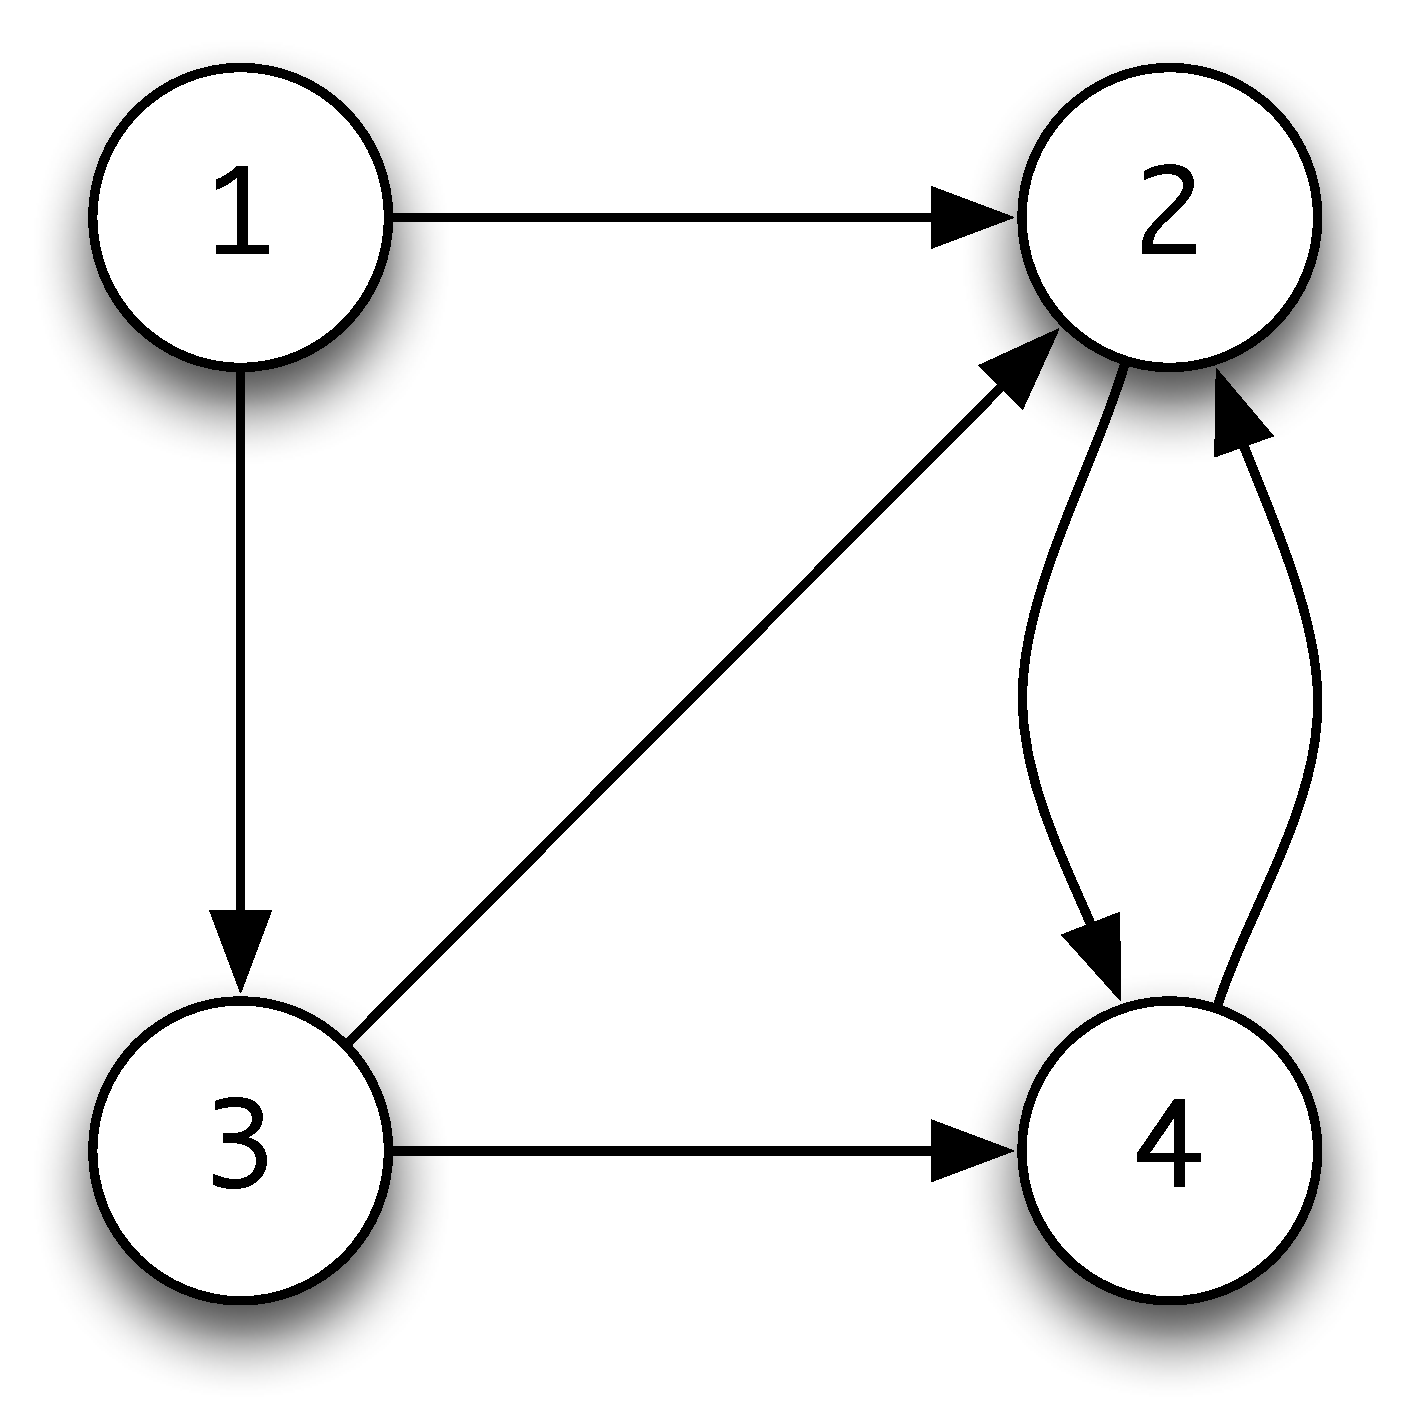
\includegraphics[width=1.5in]{Pictures/Graph.pdf}
\end{center}
where we draw an arrow joining \texttt{a} to \texttt{b} if the pair
\texttt{(a,b)} is in the relation. What then does the transitive closure represent? Two
points
\texttt{a} and \texttt{b} are related by \texttt{tClosure graph1}\minx{tClosure} if there is a
\textbf{path}\index{graph!path in} 
from \texttt{a} to \texttt{b} through the graph. For example, the pair
\texttt{(1,4)} is in the closure, since a path leads from \texttt{1} to \texttt{3}
then to \texttt{2} and finally to \texttt{4}, while the pair \texttt{(2,1)} is not in
the closure, since no path leads from \texttt{2} to \texttt{1} through the graph.

\subsection*{Strongly connected components}

A problem occurring in many different application areas, including networks
and compilers, is to find the \textbf{strongly connected components} of a graph.
\index{graph!strongly connected components}
Every graph can have its nodes split into sets or components with the
property that every node in a component is connected by a path to all
other nodes in the same component. The components of \texttt{graph1} are 
\texttt{\{1\}}, \texttt{\{3\}} and \texttt{\{2,4\}}. 

We solve the problem in two stages:
\begin{titemize}
\item we first form the relation which links points in the same component,
then
\item we form the components (or equivalence classes) generated by this
relation.
\end{titemize}
There is a path from \texttt{x} to \texttt{y} and vice versa if both \texttt{(x,y)}
and \texttt{(y,x)} are in the closure, so we define
\begin{alltt}
connect :: Ord a => Relation a -> Relation a\minx{connect}
connect rel = clos `inter` solc
              where
              clos = tClosure rel
              solc = inverse clos

inverse :: Ord a => Relation a -> Relation a\minx{inverse}
inverse = mapSet swap
          where 
          swap (x,y) = (y,x)
\end{alltt}
Now, how do we form the components given by the relation \texttt{graph1}? We start
with the set 
\begin{alltt}
\{\{1\},\{2\},\{3\},\{4\}\}
\end{alltt}
and repeatedly add the images under the relation to each of the classes,
until a fixed point is reached. In general this gives
\begin{alltt}
classes :: Ord a => Relation a -> Set (Set a)\minx{classes}
classes rel 
  = limit (addImages rel) start
    where
    start = mapSet sing (eles rel)
\end{alltt}
where the auxiliary functions used are
\begin{alltt}
eles :: Ord a => Relation a -> Set a
eles rel = mapSet fst rel `union` mapSet snd rel

addImages :: Ord a => Relation a -> Set (Set a) -> Set (Set a)
addImages rel = mapSet (addImage rel)
\end{alltt}

\subsection*{Searching in graphs}
\index{graph!search}

Many algorithms require us to \textbf{search} through the nodes of a graph: 
we might want to find a shortest path from one point to another, or to
count the number of paths between two points. 

Two general patterns of search are depth-first and breadth-first. In a
depth-first search, we explore all elements below a given child before moving
to the next child; a breadth-first search examines all the children before
examining the grandchildren, and so on. In the case of searching below node
\texttt{1} in \texttt{graph1}, the sequence \texttt{[1,2,4,3]} is depth-first (\texttt{4}
is visited before \texttt{3}), while \texttt{[1,2,3,4]} is breadth-first. These
examples show that we can characterize the searches as functions
\begin{alltt}
breadthFirst :: Ord a => Relation a -> a -> [a]
depthFirst   :: Ord a => Relation a -> a -> [a]
\end{alltt}
with  \texttt{breadthFirst graph1 1 = [1,2,3,4]}, for instance. The use of a
list in these functions is crucial -- we are not simply interested in
finding the nodes below a node (\texttt{tClosure} does this), we are interested
in the {\em order\/} in which they occur.

The essential step in both searches is to find all the descendants of a node which
have not been visited so far. We can write
\begin{alltt}
newDescs :: Ord a => Relation a -> Set a -> a -> Set a
newDescs rel st v = image rel v `diff` st
\end{alltt}
which returns the \textbf{set} of descendants of \texttt{v} in \texttt{rel} which
are not in the set \texttt{st}. Here we have a problem; the result of this
function is a set and not a list, but we require the elements in some order.
One solution is to add to the \texttt{Set} abstract data type a function
\begin{alltt}
flatten :: Set a -> [a]\hfill (setList)
flatten (Set xs) = xs
\end{alltt}
which breaks the abstraction barrier in the case of the ordered list
implementation. An alternative is to supply as a parameter a function
\begin{alltt}
minSet :: Set a -> Maybe a
\end{alltt}
which returns the minimum of a non-empty set
and which can be used in flattening a set to a list without breaking the
abstraction barrier. Unconcerned about its particular definition, we assume the existence
of a flatten function of type \texttt{(setList)}. Then we can say
\begin{alltt}
findDescs :: Ord a => Relation a -> [a] -> a -> [a]
findDescs rel xs v = flatten (newDescs rel (makeSet xs) v)
\end{alltt}

\subsubsection*{Breadth-first search}
\index{graph!search!breadth-first}

A breadth-first search involves repeatedly applying \texttt{findDescs} until a
limit is reached. The \texttt{limit} function discussed earlier will
find this, so we define
\begin{alltt}
breadthFirst :: Ord a => Relation a -> a -> [a]\minx{breadthFirst}
breadthFirst rel val
	= limit step start
	  where
	  start = [val]
	  step xs = xs ++ nub (concat (map (findDescs rel xs) xs))
\end{alltt}
A \texttt{step} performs a number of operations:
\begin{titemize}
\item First, all the descendants of
elements in \texttt{xs} which are not already in \texttt{xs} are found. This is given
by mapping \texttt{(findDescs rel xs)} along the list \texttt{xs}.
\item This list of
lists is then concatenated into a single list.  
\item Duplicates can occur
in this list, as a node may be a descendant of more than one node, 
and so any
duplicated elements must be removed. This is the effect of the library
function
\begin{alltt}\minx{nub}
nub :: Eq a => [a] -> [a]
\end{alltt}
which removes all but the first
occurrence of each element in a list.
\end{titemize}

\subsubsection*{Depth-first search}
\index{graph!search!depth-first}

How does depth-first search proceed? We first generalize the problem to
\index{generalization}
\begin{alltt}
depthSearch :: Ord a => Relation a -> a -> [a] -> [a]\minx{depthSearch}
depthFirst rel v = depthSearch rel v []
\end{alltt}
where the third argument is used to carry the list of nodes already
visited, and which are therefore not to appear in the result of the function call.
\begin{alltt}
depthSearch rel v used
        = v : depthList rel (findDescs rel used' v) used'
          where
          used' = v:used
\end{alltt}
Here we call the auxiliary function \texttt{depthList}, which finds all the
descendants of a list of nodes. 
\begin{alltt}
depthList :: Ord a => Relation a -> [a] -> [a] -> [a]

depthList rel [] used = [] 

depthList rel (val:rest) used
  = next ++ depthList rel rest (used++next)
    where
    next = if   elem val used
           then []
           else depthSearch rel val used
\end{alltt}
The definition has two equations, the first giving the trivial case where no
nodes are to be explored. In the second there are two parts to the solution:
\begin{titemize}
\item \texttt{next} gives the part of the graph accessible below \texttt{val}. This
may be \texttt{[]}, if \texttt{val} is a member of the list \texttt{used}, otherwise
\texttt{depthSearch} is called. 
\item \texttt{depthList} is then called on the tail
of the list, but with \texttt{next} appended to the list of nodes already visited.
\end{titemize}
This pair of definitions is a good example of definition by \textbf{mutual
recursion}\index{recursion!mutual}, since each calls the other. It is possible to define a single
function to perform the effect of the two, but this pair of functions seems
to express the algorithm in the most natural way.

\index{graph|)}


\begin{exercises}

\item
Calculate
\begin{alltt}
classes (connect graph1)
classes (connect graph2)
\end{alltt}
where \texttt{graph2 = graph1 \(\cup\) \{(4,3)\}}.

\item
Give calculations of 
\begin{alltt}
breadthFirst graph2 1
depthFirst graph2 1
\end{alltt}
where \texttt{graph2} is defined in the previous question.

\item
Using the searches as a model, give a function
\begin{alltt}
distance :: Eq a => Relation a -> a -> a -> Int
\end{alltt}
which gives the length of a shortest path from one node to another in a
graph. For instance,
\begin{alltt}
distance graph1 1 4 = 2
distance graph1 4 1 = 0
\end{alltt}
\texttt{0} is the result when no such path exists, or when the two nodes are
equal. 

\item
A weighted graph carries a numerical \textbf{weight} with each edge. Design a type to
model this. Give functions for breadth-first and depth-first search which
return lists of pairs. Each pair consists of a node, together with the
length of a shortest path to that node from the node at the start of the
search.

\item
A \textbf{heterogeneous} relation relates objects of different type. An
example might be the relation relating a person to their age. Design a type
to model these relations; how do you have to modify the functions defined over
\texttt{Relation a} to work over this type, if it is possible?


\item {[Harder]}
Formulate QuickCheck properties for the search functions given in this section. You should try to think of properties which are shared by all search functions, and also other properties which hold of particular search functions.





\end{exercises}



\section{Commentary}
\label{adtCommentary}

This section explores a number of issues raised by the introduction of ADTs
into our repertoire.

First, we
have not yet said anything about verification of functions over abstract
data types.
\index{proof!abstract data types and}
This is because there is nothing new to say about the {\em proof\/} of
theorems: these are proved for the implementation types exactly as we have
seen earlier. The theorems valid for an abstract data type
are precisely those which
obey the type constraints on the functions in the signature. For a queue type,
for instance, we will be able to prove that
\begin{alltt}
remQ (addQ x emptyQ) = (x , emptyQ)
\end{alltt}
by proving the appropriate result about the implementation. What would not be
valid would be an equation like 
\begin{alltt}
emptyQ = Qu []
\end{alltt}
since this breaks the information-hiding barrier and reveals something of the
implementation itself.

Next we note that our
implementation of sets gives rise to some properties which we
ought to prove, often called \textbf{invariants}.
\index{invariant}
We have assumed that our sets
are implemented as ordered lists without repetitions; we ought to prove that
each operation over our implementation preserves this property.
Both the properties of the functions, and the invariants over the implementation, can be formulated as QuickCheck properties; we leave these as exercises for the reader.

Finally, observe that both classes and
abstract data types use signatures, so it is worth surveying
their similarities and differences.
\index{classes!and ADTs}\index{signature}
\index{abstract data type!and classes}
\begin{titemize}
\item Their purposes are different: ADTs are used to provide information
hiding, and to structure programs; classes are used to overload names, to
allow the same name to be used over a class of different types.
\index{signature}
\item The signature in an ADT is associated with a single implementation
type, which may
be monomorphic or polymorphic. On the other hand, the signature in a class
will be associated with multiple instances; this is the whole point of
including classes, in fact.
\item The functions in the signature of an ADT provide the only access
to the underlying type. There is no such information hiding over classes: to
be a member of a class, a type must provide at least the types in
signature.
\end{titemize}

\begin{summary}
The abstract data types of this chapter have three
important and related properties.
\begin{titemize}
\item They provide a natural representation of a type,
which avoids being over-specific. An abstract data type carries precisely
the operations which are naturally associated with the type  and
nothing more.
\item The signature of an abstract data type
is a firm interface between the user
and the implementer: development of a system can proceed completely
independently on the two sides of the interface.
\item If the implementation of a type is to be modified,
then only the operations in the signature need to be changed;
any operation using the signature functions can be used
unchanged. We saw an example of this with search trees, when
the implementation  was modified to include size information.
\end{titemize}
We saw various examples of ADT development. Most importantly we saw
the practical example of the simulation types being designed in the three
stages suggested. First the types are named, then they are described
informally  and finally a signature is written down. After that we are able
to implement the operations of the signature as a separate task.

One of the difficulties in writing a signature is being sure that all the
relevant operations have been included; we have given a check-list of the kinds of
operations which should be present, and against which it is sensible to
evaluate any candidate signature definitions. 


\end{summary}


%\end{document}
